\chapter{Range-clone}
\label{chap:clone}

This chapter describes the range-clone operation on \bets, which can be used
to implement file or directory clones and renames in full-path-indexed \betrfs.
Unlikely a range-rename operation, which completes all its work at once,
a range-clone operation injects a new type of messages, \goto messages,
into the root node of the \bet.
The \bet then flushes \goto messages with other messages in batches, gradually
finishing the range-clone work.
Therefore, the range-clone operation fits into the write-optimized framework of
\bets.

Section~\ref{sec:rcint} describes the range-clone interface and how to implement
file or directory renames and clones in full-path-index \betrfs by calling the
range-clone operation.
Section~\ref{sec:rc} discusses how to implement the range-clone operation.
In particular, we first describes an implementation of the range-clone operation
with techniques introduced by the range-rename operation,
finishing all work on the critical path.
Then, we introduces the \goto message that delays most of the range-clone work
to the flushing process in the data structure.
At last, Section~\ref{sec:rcimp} talks about some implementation details in the
range-clone operation.

\section{The range-clone interface}
\label{sec:rcint}

\begin{table}[t]
    \centering
    \begin{tabular}{c | l}
        \hline
        Type of File System Operation & Key/Value Store Operations \\
        \hline
        \hline
        File Rename & \mdb$\rightarrow$put(\textit{dst}); \\
                    & \mdb$\rightarrow$del(\textit{src}); \\
                    & \ddb$\rightarrow$range-clone(\textit{src}, \textit{dst}, true); \\
        \hline
        Directory Rename & \mdb$\rightarrow$put(\textit{dst}); \\
                         & \mdb$\rightarrow$del(\textit{src}); \\
                         & \mdb$\rightarrow$range-clone(\textit{src/}, \textit{dst/}, true); \\
                         & \ddb$\rightarrow$range-clone(\textit{src/}, \textit{dst/}, true); \\
        \hline
        File Clone  & \mdb$\rightarrow$put(\textit{dst}); \\
                    & \ddb$\rightarrow$range-clone(\textit{src}, \textit{dst}, false); \\
        \hline
        Directory Clone  & \mdb$\rightarrow$put(\textit{dst}); \\
                         & \mdb$\rightarrow$range-clone(\textit{src/}, \textit{dst/}, false); \\
                         & \ddb$\rightarrow$range-clone(\textit{src/}, \textit{dst/}, false); \\
        \hline
    \end{tabular}
    \caption[Full-path-indexed \betrfs implements file system renames and clones with range-clone]{\label{tab:fsrc}
        Full-path-indexed \betrfs renames or clones \textit{src} to \textit{dst} by
        invoking range-clone and other operations on \bets.}
\end{table}

Range-clone is defined as
range-clone(\spre, \dpre, \delold), where \delold is a boolean value.
Range-clone(\spre, \dpre, \delold)  does the following things:
\begin{itemize}
\item it deletes all destination key/value pairs from the key/value store;
\item then, for each source key/value pair $(k,v)$ in the key/value store,
it inserts a key/value pair $(k',v)$ to the key/value store,
where $k$ is the concatenation of \spre and some suffix $s$ and $k'$ is the
concatenation of \dpre and the same suffix $s$;
\item if \delold is true, it deletes all source key/value pairs from the
key/value store.
\end{itemize}
Therefore, if \delold is true, range-clone is equivalent to range-rename;
otherwise, range-clone is range-rename without deleting source key/value pairs.

Table~\ref{tab:fsrc} summarizes how \betrfs can complete file or directory
renames and clones by invoking the range-clone operation.
Because a range-clone operation with \delold set to true is the same as a
range-rename operation,
file or directory renames in Table~\ref{tab:fsrc} are the same as those in
Table~\ref{tab:fsrr},
except using the range-clone operation instead of the range-rename operation.
And if \betrfs calls the range-clone operation but sets \delold in the
range-clone operation to false,
it keeps the source key/value pairs of metadata and data.
In such a scenario, the file system completes file or directory clones if it
doesn't call delete the metadata for the source file or directory
(in rename, this delete is not covered in the range-rename or range-clone
operation).

\section{The range-clone operation}
\label{sec:rc}

This section shows the implementation of the range-clone operation.
Because deleting source key/value pairs can be done by injecting a range-delete
message for source keys into the root node,
we set \delold to false and treat range-clone as range-clone(\spre,\dpre)
throughout the section.

Section~\ref{sec:rc:crit} shows all the changes needed if we perform all
range-clone work on the critical path.
In particular, we show that the range-clone operation can be implemented
by slightly tweaking the range-rename operation.
Then, Section~\ref{sec:rc:goto} introduces \goto messages.
A range-rename operation can return to application immediately after injecting
a \goto message into the root node.
At last, Section~\ref{sec:rc:flush} shows how \goto messages are flushed in
the data structure, gradually finishing the range-clone work.


\subsection{Range-clone, on the critical path}
\label{sec:rc:crit}

\begin{figure}
    \begin{subfigure}{\textwidth}
        \centering
        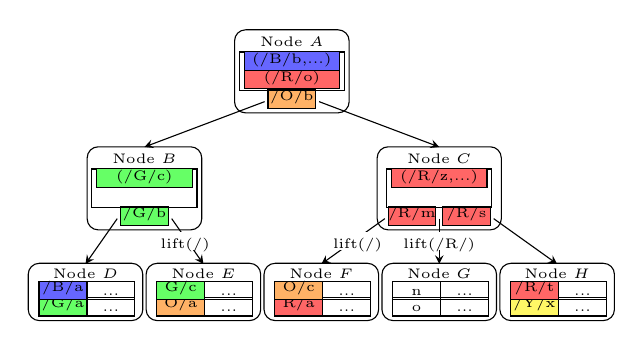
\begin{tikzpicture}[xscale=0.95, yscale=0.95]
            \node[anchor=south, rectangle, rounded corners, minimum height=.06\textwidth, minimum width=.12\textwidth, draw=black] at (0, 0) {};
            \node[anchor=south, font=\tiny] at (0, .036\textwidth) {Node $F$};
            \node[anchor=south, rectangle, minimum height=.015\textwidth, minimum width=.05\textwidth, draw=black, fill={red!60}] at (-.025\textwidth, .005\textwidth) {};
            \node[anchor=south, font=\tiny] at (-.025\textwidth, 0) {R/a};
            \node[anchor=south, rectangle, minimum height=.015\textwidth, minimum width=.05\textwidth, draw=black] at (.028\textwidth, .005\textwidth) {};
            \node[anchor=south, font=\tiny] at (.028\textwidth, 0) {...};
            \node[anchor=south, rectangle, minimum height=.015\textwidth, minimum width=.05\textwidth, draw=black, fill={orange!60}] at (-.025\textwidth, .023\textwidth) {};
            \node[anchor=south, font=\tiny] at (-.025\textwidth, .018\textwidth) {O/c};
            \node[anchor=south, rectangle, minimum height=.015\textwidth, minimum width=.05\textwidth, draw=black] at (.028\textwidth, .023\textwidth) {};
            \node[anchor=south, font=\tiny] at (.028\textwidth, .018\textwidth) {...};

            \node[anchor=south, rectangle, rounded corners, minimum height=.06\textwidth, minimum width=.12\textwidth, draw=black] at (.13\textwidth, 0) {};
            \node[anchor=south, font=\tiny] at (.13\textwidth, .036\textwidth) {Node $G$};
            \node[anchor=south, rectangle, minimum height=.015\textwidth, minimum width=.05\textwidth, draw=black] at (.105\textwidth, .005\textwidth) {};
            \node[anchor=south, font=\tiny] at (.105\textwidth, 0) {o};
            \node[anchor=south, rectangle, minimum height=.015\textwidth, minimum width=.05\textwidth, draw=black] at (.158\textwidth, .005\textwidth) {};
            \node[anchor=south, font=\tiny] at (.158\textwidth, 0) {...};
            \node[anchor=south, rectangle, minimum height=.015\textwidth, minimum width=.05\textwidth, draw=black] at (.105\textwidth, .023\textwidth) {};
            \node[anchor=south, font=\tiny] at (.105\textwidth, .018\textwidth) {n};
            \node[anchor=south, rectangle, minimum height=.015\textwidth, minimum width=.05\textwidth, draw=black] at (.158\textwidth, .023\textwidth) {};
            \node[anchor=south, font=\tiny] at (.158\textwidth, .018\textwidth) {...};

            \node[anchor=south, rectangle, rounded corners, minimum height=.06\textwidth, minimum width=.12\textwidth, draw=black] at (.26\textwidth, 0) {};
            \node[anchor=south, font=\tiny] at (.26\textwidth, .036\textwidth) {Node $H$};
            \node[anchor=south, rectangle, minimum height=.015\textwidth, minimum width=.05\textwidth, draw=black, fill={yellow!60}] at (.235\textwidth, .005\textwidth) {};
            \node[anchor=south, font=\tiny] at (.235\textwidth, 0) {/Y/x};
            \node[anchor=south, rectangle, minimum height=.015\textwidth, minimum width=.05\textwidth, draw=black] at (.288\textwidth, .005\textwidth) {};
            \node[anchor=south, font=\tiny] at (.288\textwidth, 0) {...};
            \node[anchor=south, rectangle, minimum height=.015\textwidth, minimum width=.05\textwidth, draw=black, fill={red!60}] at (.235\textwidth, .023\textwidth) {};
            \node[anchor=south, font=\tiny] at (.235\textwidth, .018\textwidth) {/R/t};
            \node[anchor=south, rectangle, minimum height=.015\textwidth, minimum width=.05\textwidth, draw=black] at (.288\textwidth, .023\textwidth) {};
            \node[anchor=south, font=\tiny] at (.288\textwidth, .018\textwidth) {...};

            \node[anchor=south, rectangle, rounded corners, minimum height=.06\textwidth, minimum width=.12\textwidth, draw=black] at (-.13\textwidth, 0) {};
            \node[anchor=south, font=\tiny] at (-.13\textwidth, .036\textwidth) {Node $E$};
            \node[anchor=south, rectangle, minimum height=.015\textwidth, minimum width=.05\textwidth, draw=black, fill={orange!60}] at (-.155\textwidth, .005\textwidth) {};
            \node[anchor=south, font=\tiny] at (-.155\textwidth, 0) {O/a};
            \node[anchor=south, rectangle, minimum height=.015\textwidth, minimum width=.05\textwidth, draw=black] at (-.102\textwidth, .005\textwidth) {};
            \node[anchor=south, font=\tiny] at (-.102\textwidth, 0) {...};
            \node[anchor=south, rectangle, minimum height=.015\textwidth, minimum width=.05\textwidth, draw=black, fill={green!60}] at (-.155\textwidth, .023\textwidth) {};
            \node[anchor=south, font=\tiny] at (-.155\textwidth, .018\textwidth) {G/c};
            \node[anchor=south, rectangle, minimum height=.015\textwidth, minimum width=.05\textwidth, draw=black] at (-.102\textwidth, .023\textwidth) {};
            \node[anchor=south, font=\tiny] at (-.102\textwidth, .018\textwidth) {...};

            \node[anchor=south, rectangle, rounded corners, minimum height=.06\textwidth, minimum width=.12\textwidth, draw=black] at (-.26\textwidth, 0) {};
            \node[anchor=south, font=\tiny] at (-.26\textwidth, .036\textwidth) {Node $D$};
            \node[anchor=south, rectangle, minimum height=.015\textwidth, minimum width=.05\textwidth, draw=black, fill={green!60}] at (-.285\textwidth, .005\textwidth) {};
            \node[anchor=south, font=\tiny] at (-.285\textwidth, 0) {/G/a};
            \node[anchor=south, rectangle, minimum height=.015\textwidth, minimum width=.05\textwidth, draw=black] at (-.232\textwidth, .005\textwidth) {};
            \node[anchor=south, font=\tiny] at (-.232\textwidth, 0) {...};
            \node[anchor=south, rectangle, minimum height=.015\textwidth, minimum width=.05\textwidth, draw=black, fill={blue!60}] at (-.285\textwidth, .023\textwidth) {};
            \node[anchor=south, font=\tiny] at (-.285\textwidth, .018\textwidth) {/B/a};
            \node[anchor=south, rectangle, minimum height=.015\textwidth, minimum width=.05\textwidth, draw=black] at (-.232\textwidth, .023\textwidth) {};
            \node[anchor=south, font=\tiny] at (-.232\textwidth, .018\textwidth) {...};

            \node[anchor=south, rectangle, rounded corners, minimum height=.087\textwidth, minimum width=.12\textwidth, draw=black] at (-.195\textwidth, .1\textwidth) {};
            \node[anchor=south, font=\tiny] at (-.195\textwidth, .163\textwidth) {Node $B$};
            \node[anchor=south, rectangle, minimum height=.015\textwidth, minimum width=.05\textwidth, draw=black, fill={green!60}] at (-.195\textwidth, .105\textwidth) {};
            \node[anchor=south, font=\tiny] at (-.195\textwidth, .1\textwidth) {/G/b};
            \node[anchor=south, rectangle, minimum height=.04\textwidth, minimum width=.11\textwidth, draw=black] at (-.195\textwidth, .125\textwidth) {};
            \node[anchor=south, rectangle, minimum height=.015\textwidth, minimum width=.1\textwidth, draw=black, fill={green!60}] at (-.195\textwidth, .147\textwidth) {};
            \node[anchor=south, font=\tiny] at  (-.195\textwidth, .141\textwidth) {\delm(/G/c)};

            \node[anchor=south, rectangle, rounded corners, minimum height=.087\textwidth, minimum width=.13\textwidth, draw=black] at (.13\textwidth, .1\textwidth) {};
            \node[anchor=south, font=\tiny] at (.13\textwidth, .163\textwidth) {Node $C$};
            \node[anchor=south, rectangle, minimum height=.015\textwidth, minimum width=.05\textwidth, draw=black, fill={red!60}] at (.1\textwidth, .105\textwidth) {};
            \node[anchor=south, font=\tiny] at (.1\textwidth, .1\textwidth) {/R/m};
            \node[anchor=south, rectangle, minimum height=.015\textwidth, minimum width=.05\textwidth, draw=black, fill={red!60}] at (.16\textwidth, .105\textwidth) {};
            \node[anchor=south, font=\tiny] at (.16\textwidth, .1\textwidth) {/R/s};
            \node[anchor=south, rectangle, minimum height=.04\textwidth, minimum width=.11\textwidth, draw=black] at (.13\textwidth, .125\textwidth) {};
            \node[anchor=south, rectangle, minimum height=.015\textwidth, minimum width=.1\textwidth, draw=black, fill={red!60}] at (.13\textwidth, .147\textwidth) {};
            \node[anchor=south, font=\tiny] at  (.13\textwidth, .141\textwidth) {\putm(/R/z,...)};

            \node[anchor=south, rectangle, rounded corners, minimum height=.087\textwidth, minimum width=.12\textwidth, draw=black] at (-.0325\textwidth, .229\textwidth) {};
            \node[anchor=south, font=\tiny] at (-.0325\textwidth, .292\textwidth) {Node $A$};
            \node[anchor=south, rectangle, minimum height=.015\textwidth, minimum width=.05\textwidth, draw=black, fill={orange!60}] at (-.0325\textwidth, .234\textwidth) {};
            \node[anchor=south, font=\tiny] at (-.0325\textwidth, .229\textwidth) {/O/b};
            \node[anchor=south, rectangle, minimum height=.04\textwidth, minimum width=.11\textwidth, draw=black] at (-.0325\textwidth, .254\textwidth) {};
            \node[anchor=south, rectangle, minimum height=.015\textwidth, minimum width=.1\textwidth, draw=black, fill={red!60}] at (-.0325\textwidth, .256\textwidth) {};
            \node[anchor=south, font=\tiny] at  (-.0325\textwidth, .25\textwidth) {\delm(/R/o)};
            \node[anchor=south, rectangle, minimum height=.015\textwidth, minimum width=.1\textwidth, draw=black, fill={blue!60}] at (-.0325\textwidth, .276\textwidth) {};
            \node[anchor=south, font=\tiny] at  (-.0325\textwidth, .27\textwidth) {\putm(/B/b,...)};

            \draw[->, >=stealth] (-.225\textwidth, .113\textwidth) -- (-.26\textwidth, .063\textwidth);
            \draw[->, >=stealth] (-.165\textwidth, .113\textwidth) -- (-.13\textwidth, .063\textwidth);
            \draw[->, >=stealth] (.13\textwidth, .113\textwidth) -- (.13\textwidth, .063\textwidth);
            \draw[->, >=stealth] (.19\textwidth, .113\textwidth) -- (.26\textwidth, .063\textwidth);
            \draw[->, >=stealth] (.07\textwidth, .113\textwidth) -- (0, .063\textwidth);
            \draw[->, >=stealth] (-.0625\textwidth, .242\textwidth) -- (-.195\textwidth, .192\textwidth);
            \draw[->, >=stealth] (-.0025\textwidth, .242\textwidth) -- (.13\textwidth, .192\textwidth);

            \node[anchor=north,rectangle, minimum height=.015\textwidth, minimum width=.05\textwidth, fill={white}] at (.13\textwidth, .099\textwidth) {};
            \node[anchor=north, font=\tiny] at (.13\textwidth, .102\textwidth) {lift(/R/)};
            \node[anchor=north,rectangle, minimum height=.015\textwidth, minimum width=.05\textwidth, fill={white}] at (.04\textwidth, .099\textwidth) {};
            \node[anchor=north, font=\tiny] at (.04\textwidth, .102\textwidth) {lift(/)};
            \node[anchor=north,rectangle, minimum height=.015\textwidth, minimum width=.05\textwidth, fill={white}] at (-.15\textwidth, .099\textwidth) {};
            \node[anchor=north, font=\tiny] at (-.15\textwidth, .102\textwidth) {lift(/)};
        \end{tikzpicture}
        \caption{\label{subfig:rc-1} The \bet before the range-clone operation.}
    \end{subfigure}
    \begin{subfigure}{\textwidth}
        \centering
        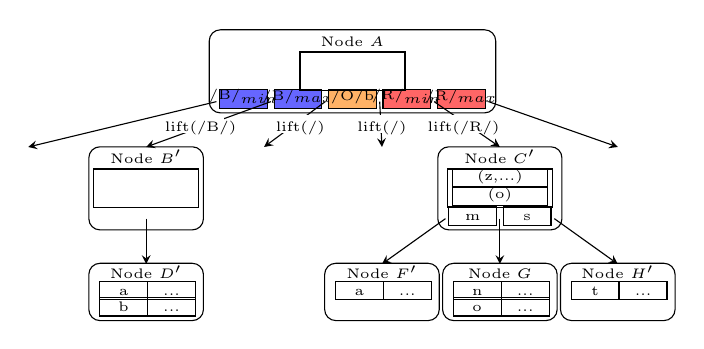
\begin{tikzpicture}[xscale=0.95, yscale=0.95]
            \node[anchor=south, rectangle, rounded corners, minimum height=.06\textwidth, minimum width=.12\textwidth, draw=black] at (0, 0) {};
            \node[anchor=south, font=\tiny] at (0, .036\textwidth) {Node $F'$};
            \node[anchor=south, rectangle, minimum height=.015\textwidth, minimum width=.05\textwidth, draw=black] at (-.025\textwidth, .023\textwidth) {};
            \node[anchor=south, font=\tiny] at (-.025\textwidth, .018\textwidth) {a};
            \node[anchor=south, rectangle, minimum height=.015\textwidth, minimum width=.05\textwidth, draw=black] at (.028\textwidth, .023\textwidth) {};
            \node[anchor=south, font=\tiny] at (.028\textwidth, .018\textwidth) {...};

            \node[anchor=south, rectangle, rounded corners, minimum height=.06\textwidth, minimum width=.12\textwidth, draw=black] at (.13\textwidth, 0) {};
            \node[anchor=south, font=\tiny] at (.13\textwidth, .036\textwidth) {Node $G$};
            \node[anchor=south, rectangle, minimum height=.015\textwidth, minimum width=.05\textwidth, draw=black] at (.105\textwidth, .005\textwidth) {};
            \node[anchor=south, font=\tiny] at (.105\textwidth, 0) {o};
            \node[anchor=south, rectangle, minimum height=.015\textwidth, minimum width=.05\textwidth, draw=black] at (.158\textwidth, .005\textwidth) {};
            \node[anchor=south, font=\tiny] at (.158\textwidth, 0) {...};
            \node[anchor=south, rectangle, minimum height=.015\textwidth, minimum width=.05\textwidth, draw=black] at (.105\textwidth, .023\textwidth) {};
            \node[anchor=south, font=\tiny] at (.105\textwidth, .018\textwidth) {n};
            \node[anchor=south, rectangle, minimum height=.015\textwidth, minimum width=.05\textwidth, draw=black] at (.158\textwidth, .023\textwidth) {};
            \node[anchor=south, font=\tiny] at (.158\textwidth, .018\textwidth) {...};

            \node[anchor=south, rectangle, rounded corners, minimum height=.06\textwidth, minimum width=.12\textwidth, draw=black] at (.26\textwidth, 0) {};
            \node[anchor=south, font=\tiny] at (.26\textwidth, .036\textwidth) {Node $H'$};
            \node[anchor=south, rectangle, minimum height=.015\textwidth, minimum width=.05\textwidth, draw=black] at (.235\textwidth, .023\textwidth) {};
            \node[anchor=south, font=\tiny] at (.235\textwidth, .018\textwidth) {t};
            \node[anchor=south, rectangle, minimum height=.015\textwidth, minimum width=.05\textwidth, draw=black] at (.288\textwidth, .023\textwidth) {};
            \node[anchor=south, font=\tiny] at (.288\textwidth, .018\textwidth) {...};

            \node[anchor=south, rectangle, rounded corners, minimum height=.06\textwidth, minimum width=.12\textwidth, draw=black] at (-.26\textwidth, 0) {};
            \node[anchor=south, font=\tiny] at (-.26\textwidth, .036\textwidth) {Node $D'$};
            \node[anchor=south, rectangle, minimum height=.015\textwidth, minimum width=.05\textwidth, draw=black] at (-.285\textwidth, .005\textwidth) {};
            \node[anchor=south, font=\tiny] at (-.285\textwidth, 0) {b};
            \node[anchor=south, rectangle, minimum height=.015\textwidth, minimum width=.05\textwidth, draw=black] at (-.232\textwidth, .005\textwidth) {};
            \node[anchor=south, font=\tiny] at (-.232\textwidth, 0) {...};
            \node[anchor=south, rectangle, minimum height=.015\textwidth, minimum width=.05\textwidth, draw=black] at (-.285\textwidth, .023\textwidth) {};
            \node[anchor=south, font=\tiny] at (-.285\textwidth, .018\textwidth) {a};
            \node[anchor=south, rectangle, minimum height=.015\textwidth, minimum width=.05\textwidth, draw=black] at (-.232\textwidth, .023\textwidth) {};
            \node[anchor=south, font=\tiny] at (-.232\textwidth, .018\textwidth) {...};

            \node[anchor=south, rectangle, rounded corners, minimum height=.087\textwidth, minimum width=.12\textwidth, draw=black] at (-.26\textwidth, .1\textwidth) {};
            \node[anchor=south, font=\tiny] at (-.26\textwidth, .163\textwidth) {Node $B'$};
            \node[anchor=south, rectangle, minimum height=.04\textwidth, minimum width=.11\textwidth, draw=black] at (-.26\textwidth, .125\textwidth) {};

            \node[anchor=south, rectangle, rounded corners, minimum height=.087\textwidth, minimum width=.13\textwidth, draw=black] at (.13\textwidth, .1\textwidth) {};
            \node[anchor=south, font=\tiny] at (.13\textwidth, .163\textwidth) {Node $C'$};
            \node[anchor=south, rectangle, minimum height=.015\textwidth, minimum width=.05\textwidth, draw=black] at (.1\textwidth, .105\textwidth) {};
            \node[anchor=south, font=\tiny] at (.1\textwidth, .1\textwidth) {m};
            \node[anchor=south, rectangle, minimum height=.015\textwidth, minimum width=.05\textwidth, draw=black] at (.16\textwidth, .105\textwidth) {};
            \node[anchor=south, font=\tiny] at (.16\textwidth, .1\textwidth) {s};
            \node[anchor=south, rectangle, minimum height=.04\textwidth, minimum width=.11\textwidth, draw=black] at (.13\textwidth, .125\textwidth) {};
            \node[anchor=south, rectangle, minimum height=.015\textwidth, minimum width=.1\textwidth, draw=black] at (.13\textwidth, .147\textwidth) {};
            \node[anchor=south, font=\tiny] at  (.13\textwidth, .141\textwidth) {\putm(z,...)};
            \node[anchor=south, rectangle, minimum height=.015\textwidth, minimum width=.1\textwidth, draw=black] at (.13\textwidth, .127\textwidth) {};
            \node[anchor=south, font=\tiny] at  (.13\textwidth, .121\textwidth) {\delm(o)};

            \node[anchor=south, rectangle, rounded corners, minimum height=.087\textwidth, minimum width=.3\textwidth, draw=black] at (-.0325\textwidth, .229\textwidth) {};
            \node[anchor=south, font=\tiny] at (-.0325\textwidth, .292\textwidth) {Node $A$};
            \node[anchor=south, rectangle, minimum height=.015\textwidth, minimum width=.05\textwidth, draw=black, fill={blue!60}] at (-.1525\textwidth, .234\textwidth) {};
            \node[anchor=south, font=\tiny] at (-.1525\textwidth, .229\textwidth) {/B/$_{min}$};
            \node[anchor=south, rectangle, minimum height=.015\textwidth, minimum width=.05\textwidth, draw=black, fill={blue!60}] at (-.0925\textwidth, .234\textwidth) {};
            \node[anchor=south, font=\tiny] at (-.0925\textwidth, .229\textwidth) {/B/$_{max}$};
            \node[anchor=south, rectangle, minimum height=.015\textwidth, minimum width=.05\textwidth, draw=black, fill={orange!60}] at (-.0325\textwidth, .234\textwidth) {};
            \node[anchor=south, font=\tiny] at (-.0325\textwidth, .229\textwidth) {/O/b};
            \node[anchor=south, rectangle, minimum height=.015\textwidth, minimum width=.05\textwidth, draw=black, fill={red!60}] at (.0275\textwidth, .234\textwidth) {};
            \node[anchor=south, font=\tiny] at (.0275\textwidth, .229\textwidth) {/R/$_{min}$};
            \node[anchor=south, rectangle, minimum height=.015\textwidth, minimum width=.05\textwidth, draw=black, fill={red!60}] at (.0875\textwidth, .234\textwidth) {};
            \node[anchor=south, font=\tiny] at (.0875\textwidth, .229\textwidth) {/R/$_{max}$};
            \node[anchor=south, rectangle, minimum height=.04\textwidth, minimum width=.11\textwidth, draw=black] at (-.0325\textwidth, .254\textwidth) {};

            \draw[->, >=stealth] (-.26\textwidth, .113\textwidth) -- (-.26\textwidth, .063\textwidth);
            \draw[->, >=stealth] (.13\textwidth, .113\textwidth) -- (.13\textwidth, .063\textwidth);
            \draw[->, >=stealth] (.19\textwidth, .113\textwidth) -- (.26\textwidth, .063\textwidth);
            \draw[->, >=stealth] (.07\textwidth, .113\textwidth) -- (0, .063\textwidth);
            \draw[->, >=stealth] (-.1825\textwidth, .242\textwidth) -- (-.39\textwidth, .192\textwidth);
            \draw[->, >=stealth] (-.1225\textwidth, .242\textwidth) -- (-.26\textwidth, .192\textwidth);
            \draw[->, >=stealth] (-.0625\textwidth, .242\textwidth) -- (-.13\textwidth, .192\textwidth);
            \draw[->, >=stealth] (-.0025\textwidth, .242\textwidth) -- (0, .192\textwidth);
            \draw[->, >=stealth] (.0575\textwidth, .242\textwidth) -- (.13\textwidth, .192\textwidth);
            \draw[->, >=stealth] (.1175\textwidth, .242\textwidth) -- (.26\textwidth, .192\textwidth);

            \node[anchor=north,rectangle, minimum height=.015\textwidth, minimum width=.05\textwidth, fill={white}] at (-.20\textwidth, .228\textwidth) {};
            \node[anchor=north, font=\tiny] at (-.20\textwidth, .231\textwidth) {lift(/B/)};
            \node[anchor=north,rectangle, minimum height=.015\textwidth, minimum width=.05\textwidth, fill={white}] at (-.09\textwidth, .228\textwidth) {};
            \node[anchor=north, font=\tiny] at (-.09\textwidth, .231\textwidth) {lift(/)};
            \node[anchor=north,rectangle, minimum height=.015\textwidth, minimum width=.05\textwidth, fill={white}] at (0, .228\textwidth) {};
            \node[anchor=north, font=\tiny] at (0, .231\textwidth) {lift(/)};
            \node[anchor=north,rectangle, minimum height=.015\textwidth, minimum width=.05\textwidth, fill={white}] at (.09\textwidth, .228\textwidth) {};
            \node[anchor=north, font=\tiny] at (.09\textwidth, .231\textwidth) {lift(/R/)};
        \end{tikzpicture}
        \caption{\label{subfig:rc-2} The range-clone operation slices out the
            source and destination subtrees.}
    \end{subfigure}
    \begin{subfigure}{\textwidth}
        \centering
        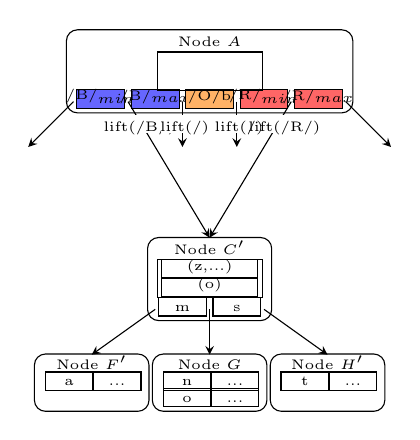
\begin{tikzpicture}[xscale=0.95, yscale=0.95]
            \node[anchor=south, rectangle, rounded corners, minimum height=.06\textwidth, minimum width=.12\textwidth, draw=black] at (-.1625\textwidth, -.1\textwidth) {};
            \node[anchor=south, font=\tiny] at (-.1625\textwidth, -.064\textwidth) {Node $F'$};
            \node[anchor=south, rectangle, minimum height=.015\textwidth, minimum width=.05\textwidth, draw=black] at (-.1875\textwidth, -.077\textwidth) {};
            \node[anchor=south, font=\tiny] at (-.1875\textwidth, -.082\textwidth) {a};
            \node[anchor=south, rectangle, minimum height=.015\textwidth, minimum width=.05\textwidth, draw=black] at (-.1345\textwidth, -.077\textwidth) {};
            \node[anchor=south, font=\tiny] at (-.1345\textwidth, -.082\textwidth) {...};

            \node[anchor=south, rectangle, rounded corners, minimum height=.06\textwidth, minimum width=.12\textwidth, draw=black] at (-.0325\textwidth, -.1\textwidth) {};
            \node[anchor=south, font=\tiny] at (-.0325\textwidth, -.064\textwidth) {Node $G$};
            \node[anchor=south, rectangle, minimum height=.015\textwidth, minimum width=.05\textwidth, draw=black] at (-.0575\textwidth, -.095\textwidth) {};
            \node[anchor=south, font=\tiny] at (-.0575\textwidth, -.1\textwidth) {o};
            \node[anchor=south, rectangle, minimum height=.015\textwidth, minimum width=.05\textwidth, draw=black] at (-.0045\textwidth, -.095\textwidth) {};
            \node[anchor=south, font=\tiny] at (-.0045\textwidth, -.1\textwidth) {...};
            \node[anchor=south, rectangle, minimum height=.015\textwidth, minimum width=.05\textwidth, draw=black] at (-.0575\textwidth, -.077\textwidth) {};
            \node[anchor=south, font=\tiny] at (-.0575\textwidth, -.082\textwidth) {n};
            \node[anchor=south, rectangle, minimum height=.015\textwidth, minimum width=.05\textwidth, draw=black] at (-.0045\textwidth, -.077\textwidth) {};
            \node[anchor=south, font=\tiny] at (-.0045\textwidth, -.082\textwidth) {...};

            \node[anchor=south, rectangle, rounded corners, minimum height=.06\textwidth, minimum width=.12\textwidth, draw=black] at (.0975\textwidth, -.1\textwidth) {};
            \node[anchor=south, font=\tiny] at (.0975\textwidth, -.064\textwidth) {Node $H'$};
            \node[anchor=south, rectangle, minimum height=.015\textwidth, minimum width=.05\textwidth, draw=black] at (.0725\textwidth, -.077\textwidth) {};
            \node[anchor=south, font=\tiny] at (.0725\textwidth, -.082\textwidth) {t};
            \node[anchor=south, rectangle, minimum height=.015\textwidth, minimum width=.05\textwidth, draw=black] at (.1255\textwidth, -.077\textwidth) {};
            \node[anchor=south, font=\tiny] at (.1255\textwidth, -.082\textwidth) {...};

            \node[anchor=south, rectangle, rounded corners, minimum height=.087\textwidth, minimum width=.13\textwidth, draw=black] at (-.0325\textwidth, 0) {};
            \node[anchor=south, font=\tiny] at (-.0325\textwidth, .063\textwidth) {Node $C'$};
            \node[anchor=south, rectangle, minimum height=.015\textwidth, minimum width=.05\textwidth, draw=black] at (-.0625\textwidth, .005\textwidth) {};
            \node[anchor=south, font=\tiny] at (-.0625\textwidth, 0) {m};
            \node[anchor=south, rectangle, minimum height=.015\textwidth, minimum width=.05\textwidth, draw=black] at (-.0025\textwidth, .005\textwidth) {};
            \node[anchor=south, font=\tiny] at (-.0025\textwidth, 0) {s};
            \node[anchor=south, rectangle, minimum height=.04\textwidth, minimum width=.11\textwidth, draw=black] at (-.0325\textwidth, .025\textwidth) {};
            \node[anchor=south, rectangle, minimum height=.015\textwidth, minimum width=.1\textwidth, draw=black] at (-.0325\textwidth, .047\textwidth) {};
            \node[anchor=south, font=\tiny] at  (-.0325\textwidth, .041\textwidth) {\putm(z,...)};
            \node[anchor=south, rectangle, minimum height=.015\textwidth, minimum width=.1\textwidth, draw=black] at (-.0325\textwidth, .027\textwidth) {};
            \node[anchor=south, font=\tiny] at  (-.0325\textwidth, .021\textwidth) {\delm(o)};

            \node[anchor=south, rectangle, rounded corners, minimum height=.087\textwidth, minimum width=.3\textwidth, draw=black] at (-.0325\textwidth, .229\textwidth) {};
            \node[anchor=south, font=\tiny] at (-.0325\textwidth, .292\textwidth) {Node $A$};
            \node[anchor=south, rectangle, minimum height=.015\textwidth, minimum width=.05\textwidth, draw=black, fill={blue!60}] at (-.1525\textwidth, .234\textwidth) {};
            \node[anchor=south, font=\tiny] at (-.1525\textwidth, .229\textwidth) {/B/$_{min}$};
            \node[anchor=south, rectangle, minimum height=.015\textwidth, minimum width=.05\textwidth, draw=black, fill={blue!60}] at (-.0925\textwidth, .234\textwidth) {};
            \node[anchor=south, font=\tiny] at (-.0925\textwidth, .229\textwidth) {/B/$_{max}$};
            \node[anchor=south, rectangle, minimum height=.015\textwidth, minimum width=.05\textwidth, draw=black, fill={orange!60}] at (-.0325\textwidth, .234\textwidth) {};
            \node[anchor=south, font=\tiny] at (-.0325\textwidth, .229\textwidth) {/O/b};
            \node[anchor=south, rectangle, minimum height=.015\textwidth, minimum width=.05\textwidth, draw=black, fill={red!60}] at (.0275\textwidth, .234\textwidth) {};
            \node[anchor=south, font=\tiny] at (.0275\textwidth, .229\textwidth) {/R/$_{min}$};
            \node[anchor=south, rectangle, minimum height=.015\textwidth, minimum width=.05\textwidth, draw=black, fill={red!60}] at (.0875\textwidth, .234\textwidth) {};
            \node[anchor=south, font=\tiny] at (.0875\textwidth, .229\textwidth) {/R/$_{max}$};
            \node[anchor=south, rectangle, minimum height=.04\textwidth, minimum width=.11\textwidth, draw=black] at (-.0325\textwidth, .254\textwidth) {};

            \draw[->, >=stealth] (-.0325\textwidth, .013\textwidth) -- (-.0325\textwidth, -.037\textwidth);
            \draw[->, >=stealth] (.0275\textwidth, .013\textwidth) -- (.0975\textwidth, -.037\textwidth);
            \draw[->, >=stealth] (-.0925\textwidth, .013\textwidth) -- (-.1625\textwidth, -.037\textwidth);
            \draw[->, >=stealth] (-.1825\textwidth, .242\textwidth) -- (-.2325\textwidth, .192\textwidth);
            \draw[->, >=stealth] (-.1225\textwidth, .242\textwidth) -- (-.0325\textwidth, .092\textwidth);
            \draw[->, >=stealth] (-.0625\textwidth, .242\textwidth) -- (-.0625\textwidth, .192\textwidth);
            \draw[->, >=stealth] (-.0025\textwidth, .242\textwidth) -- (-.0025\textwidth, .192\textwidth);
            \draw[->, >=stealth] (.0575\textwidth, .242\textwidth) -- (-.0325\textwidth, .092\textwidth);
            \draw[->, >=stealth] (.1175\textwidth, .242\textwidth) -- (.1675\textwidth, .192\textwidth);

            \node[anchor=north,rectangle, minimum height=.015\textwidth, minimum width=.05\textwidth, fill={white}] at (-.11\textwidth, .228\textwidth) {};
            \node[anchor=north, font=\tiny] at (-.11\textwidth, .231\textwidth) {lift(/B/)};
            \node[anchor=north,rectangle, minimum height=.015\textwidth, minimum width=.05\textwidth, fill={white}] at (-.06\textwidth, .228\textwidth) {};
            \node[anchor=north, font=\tiny] at (-.06\textwidth, .231\textwidth) {lift(/)};
            \node[anchor=north,rectangle, minimum height=.015\textwidth, minimum width=.05\textwidth, fill={white}] at (0, .228\textwidth) {};
            \node[anchor=north, font=\tiny] at (0, .231\textwidth) {lift(/)};
            \node[anchor=north,rectangle, minimum height=.015\textwidth, minimum width=.05\textwidth, fill={white}] at (.05\textwidth, .228\textwidth) {};
            \node[anchor=north, font=\tiny] at (.05\textwidth, .231\textwidth) {lift(/R/)};
        \end{tikzpicture}
        \caption{\label{subfig:rc-3} The range-clone operations shares the source
            subtree at both source and destination and garbage-collects the
            destination subtree.}
    \end{subfigure}
    \caption[All operations in range-clone]{\label{fig:rc}
        All operations needed in range-clone(``/R/'', ``/B/'').}
\end{figure}

The range-clone operation can be done on \bets by slightly modifying the
range-rename operation.
In particular, after slicing out the source and destination subtrees with tree
surgery,
instead of swapping the two subtrees and injecting a range-delete message
for source keys in a range-rename operation,
a range-clone operation can share the source subtree in both source and
destination and garbage-collects the destination subtree.

Figure~\ref{fig:rc} shows an example of performing the work of
range-clone(``/R/'', ``/B/'') on the lifted \bet in Figure~\ref{subfig:rc-1}.
Figure~\ref{subfig:rc-2} shows the lifted \bet after tree surgery.
Tree surgery slices out the source and destination subtrees.
This tree surgery is completely identical to that in the range-rename operation
(Figure~\ref{subfig:rr-2}).
In Figure~\ref{subfig:rc-3}, the lifted \bet garbage-collects the destination
subtree, rooted at Node $B'$, and sets the parent-to-child pointer between
``/B/$_{min}$'' and ``/B/$_{max}$'' to Node $C'$,
which is the root node of the source subtree.
The subtree rooted at Node $C'$ is now shared by two parent-to-child pointers,
and queries for
both ``/B/'' and ``/R/'' keys will fetch messages and key/value pairs in that
subtree.
However, because queries need to reconstruct the key by prepending lifted
prefixes on the root-to-leaf path, they get different keys following different
parent-to-child pointers.

Sharing a subtree among multiple parent-to-child pointers transforms a lifted
\bet into a lifted \bedag (Directed Acyclic Graph) with some constraints.
Because the \bedag is generated by sharing subtrees in a \bet,
there is still one root node in the \bedag,
which can reach all nodes in the \bedag through parent-to-child pointers.
And since the source and destination subtrees generated by tree surgery are at
the same height, the length of any root-to-leaf path in the \bedag is still
logarithmic in the size of the graph.

In a lifted \bedag, the root-to-leaf traversals of different queries may end up
reaching the same leaf node, fetching the same key/value pair.
However, because key lifting requires queries to reconstruct the full key by
concatenating lifted prefixes, different queries treat the same key/value pairs
with different prefixes.
For example, in Figure~\ref{subfig:rc-3}, queries for key ``/R/n'' and ``/B/n''
follow the same root-to-leaf path and get the same key/value pair from the
leaf node, Node $G$.
However, when waling down the tree from Node $A$ to Node $C$, the query for
key ``/R/n'' follows the parent-to-child pointer that lifts prefix ``/R/''.
Therefore, it gets key ``/R/n'' after prepending lifted prefixes along the
root-to-leaf path.
Similarly, the query for key ``/B/n'' gets a result with key ``/B/n''.

The lifted \bedag must break the sharing of a node when flushing messages
through one of its parent-to-child pointer.
Because these messages are injected into the tree after the range-clone
operation, they are not shared by all parent-to-child pointers.

The lifted \bedag maintains reference counting for each node to track the
sharing of nodes.
In particular, \fti has a node table that a maps node ID to a actual location of
the node.
We store the reference count of each node in the node table alongside
with the mapping.
Before flushing to a node, the \bedag must check the reference count of the node.
A reference count greater than 1 means the node is shared by multiple
parent-to-child pointers.
The lifted \bedag must break the sharing because other paths should not see the
messages this flush is going to inject into the node.

The lifted \bedag breaks the sharing of a node using Copy-on-Write (CoW).
For instance, after the range-clone operation, one parent of the shared node
might choose to flush its messages to the node.
At this moment, the lifted \bedag creates a new node that is identical to the
shared node, sharing the content and all children of the node.
The lifted \bedag then sets the parent-to-child pointer in the parent to the new
node and performs the flush.

\begin{figure}
    \begin{subfigure}{\textwidth}
        \centering
        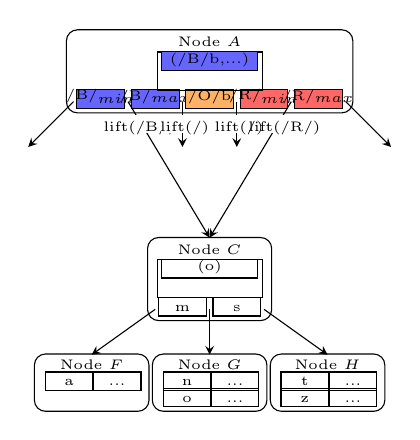
\begin{tikzpicture}[xscale=0.95, yscale=0.95]
            \node[anchor=south, rectangle, rounded corners, minimum height=.06\textwidth, minimum width=.12\textwidth, draw=black] at (-.1625\textwidth, -.1\textwidth) {};
            \node[anchor=south, font=\tiny] at (-.1625\textwidth, -.064\textwidth) {Node $F$};
            \node[anchor=south, rectangle, minimum height=.015\textwidth, minimum width=.05\textwidth, draw=black] at (-.1875\textwidth, -.077\textwidth) {};
            \node[anchor=south, font=\tiny] at (-.1875\textwidth, -.082\textwidth) {a};
            \node[anchor=south, rectangle, minimum height=.015\textwidth, minimum width=.05\textwidth, draw=black] at (-.1345\textwidth, -.077\textwidth) {};
            \node[anchor=south, font=\tiny] at (-.1345\textwidth, -.082\textwidth) {...};

            \node[anchor=south, rectangle, rounded corners, minimum height=.06\textwidth, minimum width=.12\textwidth, draw=black] at (-.0325\textwidth, -.1\textwidth) {};
            \node[anchor=south, font=\tiny] at (-.0325\textwidth, -.064\textwidth) {Node $G$};
            \node[anchor=south, rectangle, minimum height=.015\textwidth, minimum width=.05\textwidth, draw=black] at (-.0575\textwidth, -.095\textwidth) {};
            \node[anchor=south, font=\tiny] at (-.0575\textwidth, -.1\textwidth) {o};
            \node[anchor=south, rectangle, minimum height=.015\textwidth, minimum width=.05\textwidth, draw=black] at (-.0045\textwidth, -.095\textwidth) {};
            \node[anchor=south, font=\tiny] at (-.0045\textwidth, -.1\textwidth) {...};
            \node[anchor=south, rectangle, minimum height=.015\textwidth, minimum width=.05\textwidth, draw=black] at (-.0575\textwidth, -.077\textwidth) {};
            \node[anchor=south, font=\tiny] at (-.0575\textwidth, -.082\textwidth) {n};
            \node[anchor=south, rectangle, minimum height=.015\textwidth, minimum width=.05\textwidth, draw=black] at (-.0045\textwidth, -.077\textwidth) {};
            \node[anchor=south, font=\tiny] at (-.0045\textwidth, -.082\textwidth) {...};

            \node[anchor=south, rectangle, rounded corners, minimum height=.06\textwidth, minimum width=.12\textwidth, draw=black] at (.0975\textwidth, -.1\textwidth) {};
            \node[anchor=south, font=\tiny] at (.0975\textwidth, -.064\textwidth) {Node $H$};
            \node[anchor=south, rectangle, minimum height=.015\textwidth, minimum width=.05\textwidth, draw=black] at (.0725\textwidth, -.095\textwidth) {};
            \node[anchor=south, font=\tiny] at (.0725\textwidth, -.1\textwidth) {z};
            \node[anchor=south, rectangle, minimum height=.015\textwidth, minimum width=.05\textwidth, draw=black] at (.1255\textwidth, -.095\textwidth) {};
            \node[anchor=south, font=\tiny] at (.1255\textwidth, -.1\textwidth) {...};
            \node[anchor=south, rectangle, minimum height=.015\textwidth, minimum width=.05\textwidth, draw=black] at (.0725\textwidth, -.077\textwidth) {};
            \node[anchor=south, font=\tiny] at (.0725\textwidth, -.082\textwidth) {t};
            \node[anchor=south, rectangle, minimum height=.015\textwidth, minimum width=.05\textwidth, draw=black] at (.1255\textwidth, -.077\textwidth) {};
            \node[anchor=south, font=\tiny] at (.1255\textwidth, -.082\textwidth) {...};

            \node[anchor=south, rectangle, rounded corners, minimum height=.087\textwidth, minimum width=.13\textwidth, draw=black] at (-.0325\textwidth, 0) {};
            \node[anchor=south, font=\tiny] at (-.0325\textwidth, .063\textwidth) {Node $C$};
            \node[anchor=south, rectangle, minimum height=.015\textwidth, minimum width=.05\textwidth, draw=black] at (-.0625\textwidth, .005\textwidth) {};
            \node[anchor=south, font=\tiny] at (-.0625\textwidth, 0) {m};
            \node[anchor=south, rectangle, minimum height=.015\textwidth, minimum width=.05\textwidth, draw=black] at (-.0025\textwidth, .005\textwidth) {};
            \node[anchor=south, font=\tiny] at (-.0025\textwidth, 0) {s};
            \node[anchor=south, rectangle, minimum height=.04\textwidth, minimum width=.11\textwidth, draw=black] at (-.0325\textwidth, .025\textwidth) {};
            \node[anchor=south, rectangle, minimum height=.015\textwidth, minimum width=.1\textwidth, draw=black] at (-.0325\textwidth, .047\textwidth) {};
            \node[anchor=south, font=\tiny] at  (-.0325\textwidth, .041\textwidth) {\delm(o)};

            \node[anchor=south, rectangle, rounded corners, minimum height=.087\textwidth, minimum width=.3\textwidth, draw=black] at (-.0325\textwidth, .229\textwidth) {};
            \node[anchor=south, font=\tiny] at (-.0325\textwidth, .292\textwidth) {Node $A$};
            \node[anchor=south, rectangle, minimum height=.015\textwidth, minimum width=.05\textwidth, draw=black, fill={blue!60}] at (-.1525\textwidth, .234\textwidth) {};
            \node[anchor=south, font=\tiny] at (-.1525\textwidth, .229\textwidth) {/B/$_{min}$};
            \node[anchor=south, rectangle, minimum height=.015\textwidth, minimum width=.05\textwidth, draw=black, fill={blue!60}] at (-.0925\textwidth, .234\textwidth) {};
            \node[anchor=south, font=\tiny] at (-.0925\textwidth, .229\textwidth) {/B/$_{max}$};
            \node[anchor=south, rectangle, minimum height=.015\textwidth, minimum width=.05\textwidth, draw=black, fill={orange!60}] at (-.0325\textwidth, .234\textwidth) {};
            \node[anchor=south, font=\tiny] at (-.0325\textwidth, .229\textwidth) {/O/b};
            \node[anchor=south, rectangle, minimum height=.015\textwidth, minimum width=.05\textwidth, draw=black, fill={red!60}] at (.0275\textwidth, .234\textwidth) {};
            \node[anchor=south, font=\tiny] at (.0275\textwidth, .229\textwidth) {/R/$_{min}$};
            \node[anchor=south, rectangle, minimum height=.015\textwidth, minimum width=.05\textwidth, draw=black, fill={red!60}] at (.0875\textwidth, .234\textwidth) {};
            \node[anchor=south, font=\tiny] at (.0875\textwidth, .229\textwidth) {/R/$_{max}$};
            \node[anchor=south, rectangle, minimum height=.04\textwidth, minimum width=.11\textwidth, draw=black] at (-.0325\textwidth, .254\textwidth) {};
            \node[anchor=south, rectangle, minimum height=.015\textwidth, minimum width=.1\textwidth, draw=black, fill={blue!60}] at (-.0325\textwidth, .276\textwidth) {};
            \node[anchor=south, font=\tiny] at  (-.0325\textwidth, .27\textwidth) {\putm(/B/b,...)};

            \draw[->, >=stealth] (-.0325\textwidth, .013\textwidth) -- (-.0325\textwidth, -.037\textwidth);
            \draw[->, >=stealth] (.0275\textwidth, .013\textwidth) -- (.0975\textwidth, -.037\textwidth);
            \draw[->, >=stealth] (-.0925\textwidth, .013\textwidth) -- (-.1625\textwidth, -.037\textwidth);
            \draw[->, >=stealth] (-.1825\textwidth, .242\textwidth) -- (-.2325\textwidth, .192\textwidth);
            \draw[->, >=stealth] (-.1225\textwidth, .242\textwidth) -- (-.0325\textwidth, .092\textwidth);
            \draw[->, >=stealth] (-.0625\textwidth, .242\textwidth) -- (-.0625\textwidth, .192\textwidth);
            \draw[->, >=stealth] (-.0025\textwidth, .242\textwidth) -- (-.0025\textwidth, .192\textwidth);
            \draw[->, >=stealth] (.0575\textwidth, .242\textwidth) -- (-.0325\textwidth, .092\textwidth);
            \draw[->, >=stealth] (.1175\textwidth, .242\textwidth) -- (.1675\textwidth, .192\textwidth);

            \node[anchor=north,rectangle, minimum height=.015\textwidth, minimum width=.05\textwidth, fill={white}] at (-.11\textwidth, .228\textwidth) {};
            \node[anchor=north, font=\tiny] at (-.11\textwidth, .231\textwidth) {lift(/B/)};
            \node[anchor=north,rectangle, minimum height=.015\textwidth, minimum width=.05\textwidth, fill={white}] at (-.06\textwidth, .228\textwidth) {};
            \node[anchor=north, font=\tiny] at (-.06\textwidth, .231\textwidth) {lift(/)};
            \node[anchor=north,rectangle, minimum height=.015\textwidth, minimum width=.05\textwidth, fill={white}] at (0, .228\textwidth) {};
            \node[anchor=north, font=\tiny] at (0, .231\textwidth) {lift(/)};
            \node[anchor=north,rectangle, minimum height=.015\textwidth, minimum width=.05\textwidth, fill={white}] at (.05\textwidth, .228\textwidth) {};
            \node[anchor=north, font=\tiny] at (.05\textwidth, .231\textwidth) {lift(/R/)};
        \end{tikzpicture}
        \caption{\label{subfig:cow-1} Node $C$ is a shared by two
            parent-to-child pointers in Node $A$.}
    \end{subfigure}
    \begin{subfigure}{\textwidth}
        \centering
        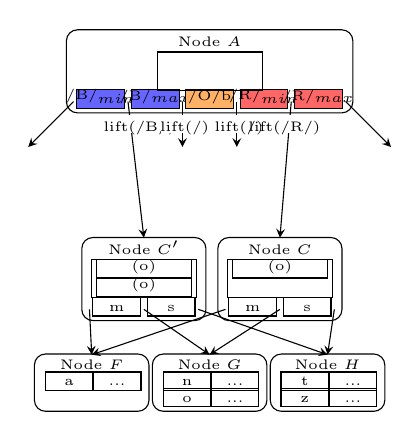
\begin{tikzpicture}[xscale=0.95, yscale=0.95]
            \node[anchor=south, rectangle, rounded corners, minimum height=.06\textwidth, minimum width=.12\textwidth, draw=black] at (-.1625\textwidth, -.1\textwidth) {};
            \node[anchor=south, font=\tiny] at (-.1625\textwidth, -.064\textwidth) {Node $F$};
            \node[anchor=south, rectangle, minimum height=.015\textwidth, minimum width=.05\textwidth, draw=black] at (-.1875\textwidth, -.077\textwidth) {};
            \node[anchor=south, font=\tiny] at (-.1875\textwidth, -.082\textwidth) {a};
            \node[anchor=south, rectangle, minimum height=.015\textwidth, minimum width=.05\textwidth, draw=black] at (-.1345\textwidth, -.077\textwidth) {};
            \node[anchor=south, font=\tiny] at (-.1345\textwidth, -.082\textwidth) {...};

            \node[anchor=south, rectangle, rounded corners, minimum height=.06\textwidth, minimum width=.12\textwidth, draw=black] at (-.0325\textwidth, -.1\textwidth) {};
            \node[anchor=south, font=\tiny] at (-.0325\textwidth, -.064\textwidth) {Node $G$};
            \node[anchor=south, rectangle, minimum height=.015\textwidth, minimum width=.05\textwidth, draw=black] at (-.0575\textwidth, -.095\textwidth) {};
            \node[anchor=south, font=\tiny] at (-.0575\textwidth, -.1\textwidth) {o};
            \node[anchor=south, rectangle, minimum height=.015\textwidth, minimum width=.05\textwidth, draw=black] at (-.0045\textwidth, -.095\textwidth) {};
            \node[anchor=south, font=\tiny] at (-.0045\textwidth, -.1\textwidth) {...};
            \node[anchor=south, rectangle, minimum height=.015\textwidth, minimum width=.05\textwidth, draw=black] at (-.0575\textwidth, -.077\textwidth) {};
            \node[anchor=south, font=\tiny] at (-.0575\textwidth, -.082\textwidth) {n};
            \node[anchor=south, rectangle, minimum height=.015\textwidth, minimum width=.05\textwidth, draw=black] at (-.0045\textwidth, -.077\textwidth) {};
            \node[anchor=south, font=\tiny] at (-.0045\textwidth, -.082\textwidth) {...};

            \node[anchor=south, rectangle, rounded corners, minimum height=.06\textwidth, minimum width=.12\textwidth, draw=black] at (.0975\textwidth, -.1\textwidth) {};
            \node[anchor=south, font=\tiny] at (.0975\textwidth, -.064\textwidth) {Node $H$};
            \node[anchor=south, rectangle, minimum height=.015\textwidth, minimum width=.05\textwidth, draw=black] at (.0725\textwidth, -.095\textwidth) {};
            \node[anchor=south, font=\tiny] at (.0725\textwidth, -.1\textwidth) {z};
            \node[anchor=south, rectangle, minimum height=.015\textwidth, minimum width=.05\textwidth, draw=black] at (.1255\textwidth, -.095\textwidth) {};
            \node[anchor=south, font=\tiny] at (.1255\textwidth, -.1\textwidth) {...};
            \node[anchor=south, rectangle, minimum height=.015\textwidth, minimum width=.05\textwidth, draw=black] at (.0725\textwidth, -.077\textwidth) {};
            \node[anchor=south, font=\tiny] at (.0725\textwidth, -.082\textwidth) {t};
            \node[anchor=south, rectangle, minimum height=.015\textwidth, minimum width=.05\textwidth, draw=black] at (.1255\textwidth, -.077\textwidth) {};
            \node[anchor=south, font=\tiny] at (.1255\textwidth, -.082\textwidth) {...};

            \node[anchor=south, rectangle, rounded corners, minimum height=.087\textwidth, minimum width=.13\textwidth, draw=black] at (.045\textwidth, 0) {};
            \node[anchor=south, font=\tiny] at (.045\textwidth, .063\textwidth) {Node $C$};
            \node[anchor=south, rectangle, minimum height=.015\textwidth, minimum width=.05\textwidth, draw=black] at (.015\textwidth, .005\textwidth) {};
            \node[anchor=south, font=\tiny] at (.015\textwidth, 0) {m};
            \node[anchor=south, rectangle, minimum height=.015\textwidth, minimum width=.05\textwidth, draw=black] at (.075\textwidth, .005\textwidth) {};
            \node[anchor=south, font=\tiny] at (.075\textwidth, 0) {s};
            \node[anchor=south, rectangle, minimum height=.04\textwidth, minimum width=.11\textwidth, draw=black] at (.045\textwidth, .025\textwidth) {};
            \node[anchor=south, rectangle, minimum height=.015\textwidth, minimum width=.1\textwidth, draw=black] at (.045\textwidth, .047\textwidth) {};
            \node[anchor=south, font=\tiny] at  (.045\textwidth, .041\textwidth) {\delm(o)};

            \node[anchor=south, rectangle, rounded corners, minimum height=.087\textwidth, minimum width=.13\textwidth, draw=black] at (-.105\textwidth, 0) {};
            \node[anchor=south, font=\tiny] at (-.105\textwidth, .063\textwidth) {Node $C'$};
            \node[anchor=south, rectangle, minimum height=.015\textwidth, minimum width=.05\textwidth, draw=black] at (-.135\textwidth, .005\textwidth) {};
            \node[anchor=south, font=\tiny] at (-.135\textwidth, 0) {m};
            \node[anchor=south, rectangle, minimum height=.015\textwidth, minimum width=.05\textwidth, draw=black] at (-.075\textwidth, .005\textwidth) {};
            \node[anchor=south, font=\tiny] at (-.075\textwidth, 0) {s};
            \node[anchor=south, rectangle, minimum height=.04\textwidth, minimum width=.11\textwidth, draw=black] at (-.105\textwidth, .025\textwidth) {};
            \node[anchor=south, rectangle, minimum height=.015\textwidth, minimum width=.1\textwidth, draw=black] at (-.105\textwidth, .047\textwidth) {};
            \node[anchor=south, font=\tiny] at  (-.105\textwidth, .041\textwidth) {\delm(o)};
            \node[anchor=south, rectangle, minimum height=.015\textwidth, minimum width=.1\textwidth, draw=black] at (-.105\textwidth, .027\textwidth) {};
            \node[anchor=south, font=\tiny] at  (-.105\textwidth, .021\textwidth) {\putm(o)};

            \node[anchor=south, rectangle, rounded corners, minimum height=.087\textwidth, minimum width=.3\textwidth, draw=black] at (-.0325\textwidth, .229\textwidth) {};
            \node[anchor=south, font=\tiny] at (-.0325\textwidth, .292\textwidth) {Node $A$};
            \node[anchor=south, rectangle, minimum height=.015\textwidth, minimum width=.05\textwidth, draw=black, fill={blue!60}] at (-.1525\textwidth, .234\textwidth) {};
            \node[anchor=south, font=\tiny] at (-.1525\textwidth, .229\textwidth) {/B/$_{min}$};
            \node[anchor=south, rectangle, minimum height=.015\textwidth, minimum width=.05\textwidth, draw=black, fill={blue!60}] at (-.0925\textwidth, .234\textwidth) {};
            \node[anchor=south, font=\tiny] at (-.0925\textwidth, .229\textwidth) {/B/$_{max}$};
            \node[anchor=south, rectangle, minimum height=.015\textwidth, minimum width=.05\textwidth, draw=black, fill={orange!60}] at (-.0325\textwidth, .234\textwidth) {};
            \node[anchor=south, font=\tiny] at (-.0325\textwidth, .229\textwidth) {/O/b};
            \node[anchor=south, rectangle, minimum height=.015\textwidth, minimum width=.05\textwidth, draw=black, fill={red!60}] at (.0275\textwidth, .234\textwidth) {};
            \node[anchor=south, font=\tiny] at (.0275\textwidth, .229\textwidth) {/R/$_{min}$};
            \node[anchor=south, rectangle, minimum height=.015\textwidth, minimum width=.05\textwidth, draw=black, fill={red!60}] at (.0875\textwidth, .234\textwidth) {};
            \node[anchor=south, font=\tiny] at (.0875\textwidth, .229\textwidth) {/R/$_{max}$};
            \node[anchor=south, rectangle, minimum height=.04\textwidth, minimum width=.11\textwidth, draw=black] at (-.0325\textwidth, .254\textwidth) {};

            \draw[->, >=stealth] (-.105\textwidth, .013\textwidth) -- (-.0325\textwidth, -.037\textwidth);
            \draw[->, >=stealth] (-.045\textwidth, .013\textwidth) -- (.0975\textwidth, -.037\textwidth);
            \draw[->, >=stealth] (-.165\textwidth, .013\textwidth) -- (-.1625\textwidth, -.037\textwidth);
            \draw[->, >=stealth] (.045\textwidth, .013\textwidth) -- (-.0325\textwidth, -.037\textwidth);
            \draw[->, >=stealth] (.105\textwidth, .013\textwidth) -- (.0975\textwidth, -.037\textwidth);
            \draw[->, >=stealth] (-.015\textwidth, .013\textwidth) -- (-.1625\textwidth, -.037\textwidth);
            \draw[->, >=stealth] (-.1825\textwidth, .242\textwidth) -- (-.2325\textwidth, .192\textwidth);
            \draw[->, >=stealth] (-.1225\textwidth, .242\textwidth) -- (-.105\textwidth, .092\textwidth);
            \draw[->, >=stealth] (-.0625\textwidth, .242\textwidth) -- (-.0625\textwidth, .192\textwidth);
            \draw[->, >=stealth] (-.0025\textwidth, .242\textwidth) -- (-.0025\textwidth, .192\textwidth);
            \draw[->, >=stealth] (.0575\textwidth, .242\textwidth) -- (.045\textwidth, .092\textwidth);
            \draw[->, >=stealth] (.1175\textwidth, .242\textwidth) -- (.1675\textwidth, .192\textwidth);

            \node[anchor=north,rectangle, minimum height=.015\textwidth, minimum width=.05\textwidth, fill={white}] at (-.11\textwidth, .228\textwidth) {};
            \node[anchor=north, font=\tiny] at (-.11\textwidth, .231\textwidth) {lift(/B/)};
            \node[anchor=north,rectangle, minimum height=.015\textwidth, minimum width=.05\textwidth, fill={white}] at (-.06\textwidth, .228\textwidth) {};
            \node[anchor=north, font=\tiny] at (-.06\textwidth, .231\textwidth) {lift(/)};
            \node[anchor=north,rectangle, minimum height=.015\textwidth, minimum width=.05\textwidth, fill={white}] at (0, .228\textwidth) {};
            \node[anchor=north, font=\tiny] at (0, .231\textwidth) {lift(/)};
            \node[anchor=north,rectangle, minimum height=.015\textwidth, minimum width=.05\textwidth, fill={white}] at (.05\textwidth, .228\textwidth) {};
            \node[anchor=north, font=\tiny] at (.05\textwidth, .231\textwidth) {lift(/R/)};
        \end{tikzpicture}
        \caption{\label{subfig:cow-2} Before Node $A$ flushes ``/B/'' messages,
            it breaks the sharing by cloning Node $C$ to Node $C'$.}
    \end{subfigure}
    \caption[\bedags break node sharing with CoW]{\label{fig:cow}
        When a parent want to flush messages to a shared node,
        it breaks the sharing by cloning the shared node.}
\end{figure}

Figure~\ref{fig:cow} shows an example of the CoW process.
In Figure~\ref{subfig:cow-1}, Node $A$ has two parent-to-child pointers to
Node $C$.
The reference count of Node $C'$ is 2 and
Node $F$, $G$ and $H$ have reference count 1
(assume nodes omitted in the figure don't have parent-to-child pointers
to nodes shown in the figure).
When Node $A$ wants to flush messages with through the parent-to-child pointer
between ``/B/$_{min}$'' and ``/B/$_{max}$'',
it finds out that Node $C$ is a shared node because its reference count is
greater than 1.
Therefore, it clones Node $C$ to break the sharing.
As shown in Figure~\ref{subfig:cow-2}, the \bedag creates a new Node $C'$,
identical to Node $C$.
Now, both Node $C'$ and $C''$ have reference count 1, while Node $F$, $G$ and
$H$ have reference count 2.
With the sharing broken, the \bedag can flush message \putm(``/B/b'',...) from
Node $A$ to Node $C'$ without affecting the other root-to-leaf path that
includes Node $C$.

\subsection{Range-clone with \goto messages}
\label{sec:rc:goto}

Instead of performing all works on the critical path, range-clone can use a
new type of messages, the \goto message, that delays tree surgery
in the lifted \bedag.

\paragraph{The \goto message.}
A \goto message consists of 3 parts: a \dpre, a \spre, a node ID
(with its height in the \bedag).
When a query visits a node during its root-to-leaf traversal, it must check
\goto messages.
If the \dpre of a \goto message matches the search key, the query should follow
the \goto message, instead of the parent-to-child pointer in the node.
In other words, the next node this query visit should be the node whose node ID
is in the \goto message.
Also, the query should update its search key by changing the prefix from \dpre
to \spre.
If the query finds multiple \goto messages matching its search key, it follows
the \goto message with the latest timestamp.

A \goto message serves as an additional parent-to-child pointer in the node with
a \xf (translate-and-filter) function.
The \xf function not only translates search keys for queries by updating their
prefix, but also filters out out-of-range keys in nodes that would be visited
following the \goto message.
Consider a query for key ``/B/b'' visits Node $A$ in its root-to-leaf traversal,
and finds a \goto message, \goto(``/B/'', ``/R'', $C$), in node $A$.
This query should follow the \goto message and visit Node $C$,
instead of normal children of Node $A$.
Additionally, the \goto message acts as a \xf function that translates the
search key ``/B/b'' to ``/R/b'' and bounds the query result to
(``/R/$_{min}$'', ``/R/$_{max}$''),
i.e., the query should not return any result with a key out of that range
(a range query for key ``/R/b'' may return a key/value pair whose key doesn't
have ``/R/'' prefix).

Because a \goto message redirects queries whose search keys have a certain
prefix, it also acts as a range-delete message that invalidates all old messages
and key/value pairs following other pointers (normal parent-to-child pointers
and older \goto messages).
Thus, if we set the node ID in a \goto message to a special value
(e.g., 0), the \goto message acts as a range-delete message.
Therefore, we can use \goto message to implement range-delete.

\begin{figure}
    \begin{subfigure}{\textwidth}
        \centering
        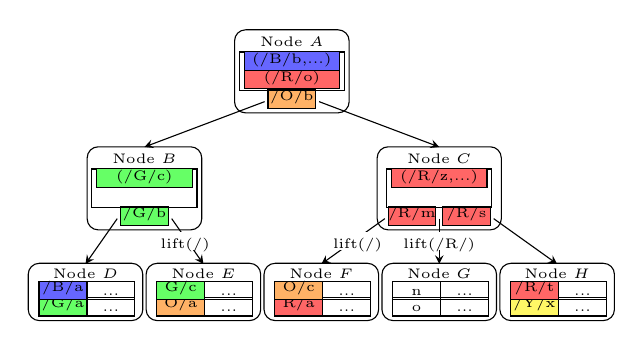
\begin{tikzpicture}[xscale=0.95, yscale=0.95]
            \node[anchor=south, rectangle, rounded corners, minimum height=.06\textwidth, minimum width=.12\textwidth, draw=black] at (0, 0) {};
            \node[anchor=south, font=\tiny] at (0, .036\textwidth) {Node $F$};
            \node[anchor=south, rectangle, minimum height=.015\textwidth, minimum width=.05\textwidth, draw=black, fill={red!60}] at (-.025\textwidth, .005\textwidth) {};
            \node[anchor=south, font=\tiny] at (-.025\textwidth, 0) {R/a};
            \node[anchor=south, rectangle, minimum height=.015\textwidth, minimum width=.05\textwidth, draw=black] at (.028\textwidth, .005\textwidth) {};
            \node[anchor=south, font=\tiny] at (.028\textwidth, 0) {...};
            \node[anchor=south, rectangle, minimum height=.015\textwidth, minimum width=.05\textwidth, draw=black, fill={orange!60}] at (-.025\textwidth, .023\textwidth) {};
            \node[anchor=south, font=\tiny] at (-.025\textwidth, .018\textwidth) {O/c};
            \node[anchor=south, rectangle, minimum height=.015\textwidth, minimum width=.05\textwidth, draw=black] at (.028\textwidth, .023\textwidth) {};
            \node[anchor=south, font=\tiny] at (.028\textwidth, .018\textwidth) {...};

            \node[anchor=south, rectangle, rounded corners, minimum height=.06\textwidth, minimum width=.12\textwidth, draw=black] at (.13\textwidth, 0) {};
            \node[anchor=south, font=\tiny] at (.13\textwidth, .036\textwidth) {Node $G$};
            \node[anchor=south, rectangle, minimum height=.015\textwidth, minimum width=.05\textwidth, draw=black] at (.105\textwidth, .005\textwidth) {};
            \node[anchor=south, font=\tiny] at (.105\textwidth, 0) {o};
            \node[anchor=south, rectangle, minimum height=.015\textwidth, minimum width=.05\textwidth, draw=black] at (.158\textwidth, .005\textwidth) {};
            \node[anchor=south, font=\tiny] at (.158\textwidth, 0) {...};
            \node[anchor=south, rectangle, minimum height=.015\textwidth, minimum width=.05\textwidth, draw=black] at (.105\textwidth, .023\textwidth) {};
            \node[anchor=south, font=\tiny] at (.105\textwidth, .018\textwidth) {n};
            \node[anchor=south, rectangle, minimum height=.015\textwidth, minimum width=.05\textwidth, draw=black] at (.158\textwidth, .023\textwidth) {};
            \node[anchor=south, font=\tiny] at (.158\textwidth, .018\textwidth) {...};

            \node[anchor=south, rectangle, rounded corners, minimum height=.06\textwidth, minimum width=.12\textwidth, draw=black] at (.26\textwidth, 0) {};
            \node[anchor=south, font=\tiny] at (.26\textwidth, .036\textwidth) {Node $H$};
            \node[anchor=south, rectangle, minimum height=.015\textwidth, minimum width=.05\textwidth, draw=black, fill={yellow!60}] at (.235\textwidth, .005\textwidth) {};
            \node[anchor=south, font=\tiny] at (.235\textwidth, 0) {/Y/x};
            \node[anchor=south, rectangle, minimum height=.015\textwidth, minimum width=.05\textwidth, draw=black] at (.288\textwidth, .005\textwidth) {};
            \node[anchor=south, font=\tiny] at (.288\textwidth, 0) {...};
            \node[anchor=south, rectangle, minimum height=.015\textwidth, minimum width=.05\textwidth, draw=black, fill={red!60}] at (.235\textwidth, .023\textwidth) {};
            \node[anchor=south, font=\tiny] at (.235\textwidth, .018\textwidth) {/R/t};
            \node[anchor=south, rectangle, minimum height=.015\textwidth, minimum width=.05\textwidth, draw=black] at (.288\textwidth, .023\textwidth) {};
            \node[anchor=south, font=\tiny] at (.288\textwidth, .018\textwidth) {...};

            \node[anchor=south, rectangle, rounded corners, minimum height=.06\textwidth, minimum width=.12\textwidth, draw=black] at (-.13\textwidth, 0) {};
            \node[anchor=south, font=\tiny] at (-.13\textwidth, .036\textwidth) {Node $E$};
            \node[anchor=south, rectangle, minimum height=.015\textwidth, minimum width=.05\textwidth, draw=black, fill={orange!60}] at (-.155\textwidth, .005\textwidth) {};
            \node[anchor=south, font=\tiny] at (-.155\textwidth, 0) {O/a};
            \node[anchor=south, rectangle, minimum height=.015\textwidth, minimum width=.05\textwidth, draw=black] at (-.102\textwidth, .005\textwidth) {};
            \node[anchor=south, font=\tiny] at (-.102\textwidth, 0) {...};
            \node[anchor=south, rectangle, minimum height=.015\textwidth, minimum width=.05\textwidth, draw=black, fill={green!60}] at (-.155\textwidth, .023\textwidth) {};
            \node[anchor=south, font=\tiny] at (-.155\textwidth, .018\textwidth) {G/c};
            \node[anchor=south, rectangle, minimum height=.015\textwidth, minimum width=.05\textwidth, draw=black] at (-.102\textwidth, .023\textwidth) {};
            \node[anchor=south, font=\tiny] at (-.102\textwidth, .018\textwidth) {...};

            \node[anchor=south, rectangle, rounded corners, minimum height=.06\textwidth, minimum width=.12\textwidth, draw=black] at (-.26\textwidth, 0) {};
            \node[anchor=south, font=\tiny] at (-.26\textwidth, .036\textwidth) {Node $D$};
            \node[anchor=south, rectangle, minimum height=.015\textwidth, minimum width=.05\textwidth, draw=black, fill={green!60}] at (-.285\textwidth, .005\textwidth) {};
            \node[anchor=south, font=\tiny] at (-.285\textwidth, 0) {/G/a};
            \node[anchor=south, rectangle, minimum height=.015\textwidth, minimum width=.05\textwidth, draw=black] at (-.232\textwidth, .005\textwidth) {};
            \node[anchor=south, font=\tiny] at (-.232\textwidth, 0) {...};
            \node[anchor=south, rectangle, minimum height=.015\textwidth, minimum width=.05\textwidth, draw=black, fill={blue!60}] at (-.285\textwidth, .023\textwidth) {};
            \node[anchor=south, font=\tiny] at (-.285\textwidth, .018\textwidth) {/B/a};
            \node[anchor=south, rectangle, minimum height=.015\textwidth, minimum width=.05\textwidth, draw=black] at (-.232\textwidth, .023\textwidth) {};
            \node[anchor=south, font=\tiny] at (-.232\textwidth, .018\textwidth) {...};

            \node[anchor=south, rectangle, rounded corners, minimum height=.087\textwidth, minimum width=.12\textwidth, draw=black] at (-.195\textwidth, .1\textwidth) {};
            \node[anchor=south, font=\tiny] at (-.195\textwidth, .163\textwidth) {Node $B$};
            \node[anchor=south, rectangle, minimum height=.015\textwidth, minimum width=.05\textwidth, draw=black, fill={green!60}] at (-.195\textwidth, .105\textwidth) {};
            \node[anchor=south, font=\tiny] at (-.195\textwidth, .1\textwidth) {/G/b};
            \node[anchor=south, rectangle, minimum height=.04\textwidth, minimum width=.11\textwidth, draw=black] at (-.195\textwidth, .125\textwidth) {};
            \node[anchor=south, rectangle, minimum height=.015\textwidth, minimum width=.1\textwidth, draw=black, fill={green!60}] at (-.195\textwidth, .147\textwidth) {};
            \node[anchor=south, font=\tiny] at  (-.195\textwidth, .141\textwidth) {\delm(/G/c)};

            \node[anchor=south, rectangle, rounded corners, minimum height=.087\textwidth, minimum width=.13\textwidth, draw=black] at (.13\textwidth, .1\textwidth) {};
            \node[anchor=south, font=\tiny] at (.13\textwidth, .163\textwidth) {Node $C$};
            \node[anchor=south, rectangle, minimum height=.015\textwidth, minimum width=.05\textwidth, draw=black, fill={red!60}] at (.1\textwidth, .105\textwidth) {};
            \node[anchor=south, font=\tiny] at (.1\textwidth, .1\textwidth) {/R/m};
            \node[anchor=south, rectangle, minimum height=.015\textwidth, minimum width=.05\textwidth, draw=black, fill={red!60}] at (.16\textwidth, .105\textwidth) {};
            \node[anchor=south, font=\tiny] at (.16\textwidth, .1\textwidth) {/R/s};
            \node[anchor=south, rectangle, minimum height=.04\textwidth, minimum width=.11\textwidth, draw=black] at (.13\textwidth, .125\textwidth) {};
            \node[anchor=south, rectangle, minimum height=.015\textwidth, minimum width=.1\textwidth, draw=black, fill={red!60}] at (.13\textwidth, .147\textwidth) {};
            \node[anchor=south, font=\tiny] at  (.13\textwidth, .141\textwidth) {\putm(/R/z,...)};

            \node[anchor=south, rectangle, rounded corners, minimum height=.087\textwidth, minimum width=.12\textwidth, draw=black] at (-.0325\textwidth, .229\textwidth) {};
            \node[anchor=south, font=\tiny] at (-.0325\textwidth, .292\textwidth) {Node $A$};
            \node[anchor=south, rectangle, minimum height=.015\textwidth, minimum width=.05\textwidth, draw=black, fill={orange!60}] at (-.0325\textwidth, .234\textwidth) {};
            \node[anchor=south, font=\tiny] at (-.0325\textwidth, .229\textwidth) {/O/b};
            \node[anchor=south, rectangle, minimum height=.04\textwidth, minimum width=.11\textwidth, draw=black] at (-.0325\textwidth, .254\textwidth) {};
            \node[anchor=south, rectangle, minimum height=.015\textwidth, minimum width=.1\textwidth, draw=black, fill={red!60}] at (-.0325\textwidth, .256\textwidth) {};
            \node[anchor=south, font=\tiny] at  (-.0325\textwidth, .25\textwidth) {\delm(/R/o)};
            \node[anchor=south, rectangle, minimum height=.015\textwidth, minimum width=.1\textwidth, draw=black, fill={blue!60}] at (-.0325\textwidth, .276\textwidth) {};
            \node[anchor=south, font=\tiny] at  (-.0325\textwidth, .27\textwidth) {\putm(/B/b,...)};

            \draw[->, >=stealth] (-.225\textwidth, .113\textwidth) -- (-.26\textwidth, .063\textwidth);
            \draw[->, >=stealth] (-.165\textwidth, .113\textwidth) -- (-.13\textwidth, .063\textwidth);
            \draw[->, >=stealth] (.13\textwidth, .113\textwidth) -- (.13\textwidth, .063\textwidth);
            \draw[->, >=stealth] (.19\textwidth, .113\textwidth) -- (.26\textwidth, .063\textwidth);
            \draw[->, >=stealth] (.07\textwidth, .113\textwidth) -- (0, .063\textwidth);
            \draw[->, >=stealth] (-.0625\textwidth, .242\textwidth) -- (-.195\textwidth, .192\textwidth);
            \draw[->, >=stealth] (-.0025\textwidth, .242\textwidth) -- (.13\textwidth, .192\textwidth);

            \node[anchor=north,rectangle, minimum height=.015\textwidth, minimum width=.05\textwidth, fill={white}] at (.13\textwidth, .099\textwidth) {};
            \node[anchor=north, font=\tiny] at (.13\textwidth, .102\textwidth) {lift(/R/)};
            \node[anchor=north,rectangle, minimum height=.015\textwidth, minimum width=.05\textwidth, fill={white}] at (.04\textwidth, .099\textwidth) {};
            \node[anchor=north, font=\tiny] at (.04\textwidth, .102\textwidth) {lift(/)};
            \node[anchor=north,rectangle, minimum height=.015\textwidth, minimum width=.05\textwidth, fill={white}] at (-.15\textwidth, .099\textwidth) {};
            \node[anchor=north, font=\tiny] at (-.15\textwidth, .102\textwidth) {lift(/)};
        \end{tikzpicture}
        \caption{\label{subfig:goto-1} The \bet before the range-clone.}
    \end{subfigure}
    \begin{subfigure}{\textwidth}
        \centering
        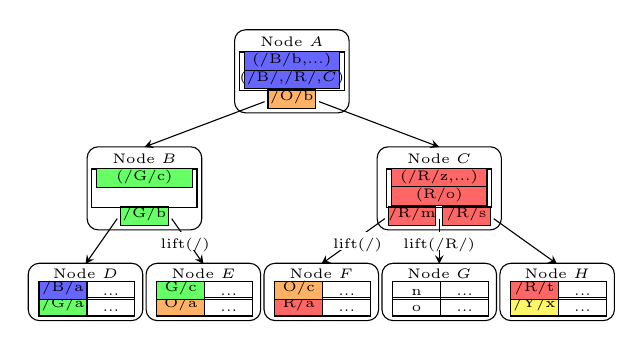
\begin{tikzpicture}[xscale=0.95, yscale=0.95]
            \node[anchor=south, rectangle, rounded corners, minimum height=.06\textwidth, minimum width=.12\textwidth, draw=black] at (0, 0) {};
            \node[anchor=south, font=\tiny] at (0, .036\textwidth) {Node $F$};
            \node[anchor=south, rectangle, minimum height=.015\textwidth, minimum width=.05\textwidth, draw=black, fill={red!60}] at (-.025\textwidth, .005\textwidth) {};
            \node[anchor=south, font=\tiny] at (-.025\textwidth, 0) {R/a};
            \node[anchor=south, rectangle, minimum height=.015\textwidth, minimum width=.05\textwidth, draw=black] at (.028\textwidth, .005\textwidth) {};
            \node[anchor=south, font=\tiny] at (.028\textwidth, 0) {...};
            \node[anchor=south, rectangle, minimum height=.015\textwidth, minimum width=.05\textwidth, draw=black, fill={orange!60}] at (-.025\textwidth, .023\textwidth) {};
            \node[anchor=south, font=\tiny] at (-.025\textwidth, .018\textwidth) {O/c};
            \node[anchor=south, rectangle, minimum height=.015\textwidth, minimum width=.05\textwidth, draw=black] at (.028\textwidth, .023\textwidth) {};
            \node[anchor=south, font=\tiny] at (.028\textwidth, .018\textwidth) {...};

            \node[anchor=south, rectangle, rounded corners, minimum height=.06\textwidth, minimum width=.12\textwidth, draw=black] at (.13\textwidth, 0) {};
            \node[anchor=south, font=\tiny] at (.13\textwidth, .036\textwidth) {Node $G$};
            \node[anchor=south, rectangle, minimum height=.015\textwidth, minimum width=.05\textwidth, draw=black] at (.105\textwidth, .005\textwidth) {};
            \node[anchor=south, font=\tiny] at (.105\textwidth, 0) {o};
            \node[anchor=south, rectangle, minimum height=.015\textwidth, minimum width=.05\textwidth, draw=black] at (.158\textwidth, .005\textwidth) {};
            \node[anchor=south, font=\tiny] at (.158\textwidth, 0) {...};
            \node[anchor=south, rectangle, minimum height=.015\textwidth, minimum width=.05\textwidth, draw=black] at (.105\textwidth, .023\textwidth) {};
            \node[anchor=south, font=\tiny] at (.105\textwidth, .018\textwidth) {n};
            \node[anchor=south, rectangle, minimum height=.015\textwidth, minimum width=.05\textwidth, draw=black] at (.158\textwidth, .023\textwidth) {};
            \node[anchor=south, font=\tiny] at (.158\textwidth, .018\textwidth) {...};

            \node[anchor=south, rectangle, rounded corners, minimum height=.06\textwidth, minimum width=.12\textwidth, draw=black] at (.26\textwidth, 0) {};
            \node[anchor=south, font=\tiny] at (.26\textwidth, .036\textwidth) {Node $H$};
            \node[anchor=south, rectangle, minimum height=.015\textwidth, minimum width=.05\textwidth, draw=black, fill={yellow!60}] at (.235\textwidth, .005\textwidth) {};
            \node[anchor=south, font=\tiny] at (.235\textwidth, 0) {/Y/x};
            \node[anchor=south, rectangle, minimum height=.015\textwidth, minimum width=.05\textwidth, draw=black] at (.288\textwidth, .005\textwidth) {};
            \node[anchor=south, font=\tiny] at (.288\textwidth, 0) {...};
            \node[anchor=south, rectangle, minimum height=.015\textwidth, minimum width=.05\textwidth, draw=black, fill={red!60}] at (.235\textwidth, .023\textwidth) {};
            \node[anchor=south, font=\tiny] at (.235\textwidth, .018\textwidth) {/R/t};
            \node[anchor=south, rectangle, minimum height=.015\textwidth, minimum width=.05\textwidth, draw=black] at (.288\textwidth, .023\textwidth) {};
            \node[anchor=south, font=\tiny] at (.288\textwidth, .018\textwidth) {...};

            \node[anchor=south, rectangle, rounded corners, minimum height=.06\textwidth, minimum width=.12\textwidth, draw=black] at (-.13\textwidth, 0) {};
            \node[anchor=south, font=\tiny] at (-.13\textwidth, .036\textwidth) {Node $E$};
            \node[anchor=south, rectangle, minimum height=.015\textwidth, minimum width=.05\textwidth, draw=black, fill={orange!60}] at (-.155\textwidth, .005\textwidth) {};
            \node[anchor=south, font=\tiny] at (-.155\textwidth, 0) {O/a};
            \node[anchor=south, rectangle, minimum height=.015\textwidth, minimum width=.05\textwidth, draw=black] at (-.102\textwidth, .005\textwidth) {};
            \node[anchor=south, font=\tiny] at (-.102\textwidth, 0) {...};
            \node[anchor=south, rectangle, minimum height=.015\textwidth, minimum width=.05\textwidth, draw=black, fill={green!60}] at (-.155\textwidth, .023\textwidth) {};
            \node[anchor=south, font=\tiny] at (-.155\textwidth, .018\textwidth) {G/c};
            \node[anchor=south, rectangle, minimum height=.015\textwidth, minimum width=.05\textwidth, draw=black] at (-.102\textwidth, .023\textwidth) {};
            \node[anchor=south, font=\tiny] at (-.102\textwidth, .018\textwidth) {...};

            \node[anchor=south, rectangle, rounded corners, minimum height=.06\textwidth, minimum width=.12\textwidth, draw=black] at (-.26\textwidth, 0) {};
            \node[anchor=south, font=\tiny] at (-.26\textwidth, .036\textwidth) {Node $D$};
            \node[anchor=south, rectangle, minimum height=.015\textwidth, minimum width=.05\textwidth, draw=black, fill={green!60}] at (-.285\textwidth, .005\textwidth) {};
            \node[anchor=south, font=\tiny] at (-.285\textwidth, 0) {/G/a};
            \node[anchor=south, rectangle, minimum height=.015\textwidth, minimum width=.05\textwidth, draw=black] at (-.232\textwidth, .005\textwidth) {};
            \node[anchor=south, font=\tiny] at (-.232\textwidth, 0) {...};
            \node[anchor=south, rectangle, minimum height=.015\textwidth, minimum width=.05\textwidth, draw=black, fill={blue!60}] at (-.285\textwidth, .023\textwidth) {};
            \node[anchor=south, font=\tiny] at (-.285\textwidth, .018\textwidth) {/B/a};
            \node[anchor=south, rectangle, minimum height=.015\textwidth, minimum width=.05\textwidth, draw=black] at (-.232\textwidth, .023\textwidth) {};
            \node[anchor=south, font=\tiny] at (-.232\textwidth, .018\textwidth) {...};

            \node[anchor=south, rectangle, rounded corners, minimum height=.087\textwidth, minimum width=.12\textwidth, draw=black] at (-.195\textwidth, .1\textwidth) {};
            \node[anchor=south, font=\tiny] at (-.195\textwidth, .163\textwidth) {Node $B$};
            \node[anchor=south, rectangle, minimum height=.015\textwidth, minimum width=.05\textwidth, draw=black, fill={green!60}] at (-.195\textwidth, .105\textwidth) {};
            \node[anchor=south, font=\tiny] at (-.195\textwidth, .1\textwidth) {/G/b};
            \node[anchor=south, rectangle, minimum height=.04\textwidth, minimum width=.11\textwidth, draw=black] at (-.195\textwidth, .125\textwidth) {};
            \node[anchor=south, rectangle, minimum height=.015\textwidth, minimum width=.1\textwidth, draw=black, fill={green!60}] at (-.195\textwidth, .147\textwidth) {};
            \node[anchor=south, font=\tiny] at  (-.195\textwidth, .141\textwidth) {\delm(/G/c)};

            \node[anchor=south, rectangle, rounded corners, minimum height=.087\textwidth, minimum width=.13\textwidth, draw=black] at (.13\textwidth, .1\textwidth) {};
            \node[anchor=south, font=\tiny] at (.13\textwidth, .163\textwidth) {Node $C$};
            \node[anchor=south, rectangle, minimum height=.015\textwidth, minimum width=.05\textwidth, draw=black, fill={red!60}] at (.1\textwidth, .105\textwidth) {};
            \node[anchor=south, font=\tiny] at (.1\textwidth, .1\textwidth) {/R/m};
            \node[anchor=south, rectangle, minimum height=.015\textwidth, minimum width=.05\textwidth, draw=black, fill={red!60}] at (.16\textwidth, .105\textwidth) {};
            \node[anchor=south, font=\tiny] at (.16\textwidth, .1\textwidth) {/R/s};
            \node[anchor=south, rectangle, minimum height=.04\textwidth, minimum width=.11\textwidth, draw=black] at (.13\textwidth, .125\textwidth) {};
            \node[anchor=south, rectangle, minimum height=.015\textwidth, minimum width=.1\textwidth, draw=black, fill={red!60}] at (.13\textwidth, .147\textwidth) {};
            \node[anchor=south, font=\tiny] at  (.13\textwidth, .141\textwidth) {\putm(/R/z,...)};
            \node[anchor=south, rectangle, minimum height=.015\textwidth, minimum width=.1\textwidth, draw=black, fill={red!60}] at (.13\textwidth, .127\textwidth) {};
            \node[anchor=south, font=\tiny] at  (.13\textwidth, .121\textwidth) {\delm(R/o)};

            \node[anchor=south, rectangle, rounded corners, minimum height=.087\textwidth, minimum width=.12\textwidth, draw=black] at (-.0325\textwidth, .229\textwidth) {};
            \node[anchor=south, font=\tiny] at (-.0325\textwidth, .292\textwidth) {Node $A$};
            \node[anchor=south, rectangle, minimum height=.015\textwidth, minimum width=.05\textwidth, draw=black, fill={orange!60}] at (-.0325\textwidth, .234\textwidth) {};
            \node[anchor=south, font=\tiny] at (-.0325\textwidth, .229\textwidth) {/O/b};
            \node[anchor=south, rectangle, minimum height=.04\textwidth, minimum width=.11\textwidth, draw=black] at (-.0325\textwidth, .254\textwidth) {};
            \node[anchor=south, rectangle, minimum height=.015\textwidth, minimum width=.1\textwidth, draw=black, fill={blue!60}] at (-.0325\textwidth, .256\textwidth) {};
            \node[anchor=south, font=\tiny] at  (-.0325\textwidth, .25\textwidth) {\goto(/B/,/R/,$C$)};
            \node[anchor=south, rectangle, minimum height=.015\textwidth, minimum width=.1\textwidth, draw=black, fill={blue!60}] at (-.0325\textwidth, .276\textwidth) {};
            \node[anchor=south, font=\tiny] at  (-.0325\textwidth, .27\textwidth) {\putm(/B/b,...)};

            \draw[->, >=stealth] (-.225\textwidth, .113\textwidth) -- (-.26\textwidth, .063\textwidth);
            \draw[->, >=stealth] (-.165\textwidth, .113\textwidth) -- (-.13\textwidth, .063\textwidth);
            \draw[->, >=stealth] (.13\textwidth, .113\textwidth) -- (.13\textwidth, .063\textwidth);
            \draw[->, >=stealth] (.19\textwidth, .113\textwidth) -- (.26\textwidth, .063\textwidth);
            \draw[->, >=stealth] (.07\textwidth, .113\textwidth) -- (0, .063\textwidth);
            \draw[->, >=stealth] (-.0625\textwidth, .242\textwidth) -- (-.195\textwidth, .192\textwidth);
            \draw[->, >=stealth] (-.0025\textwidth, .242\textwidth) -- (.13\textwidth, .192\textwidth);

            \node[anchor=north,rectangle, minimum height=.015\textwidth, minimum width=.05\textwidth, fill={white}] at (.13\textwidth, .099\textwidth) {};
            \node[anchor=north, font=\tiny] at (.13\textwidth, .102\textwidth) {lift(/R/)};
            \node[anchor=north,rectangle, minimum height=.015\textwidth, minimum width=.05\textwidth, fill={white}] at (.04\textwidth, .099\textwidth) {};
            \node[anchor=north, font=\tiny] at (.04\textwidth, .102\textwidth) {lift(/)};
            \node[anchor=north,rectangle, minimum height=.015\textwidth, minimum width=.05\textwidth, fill={white}] at (-.15\textwidth, .099\textwidth) {};
            \node[anchor=north, font=\tiny] at (-.15\textwidth, .102\textwidth) {lift(/)};
        \end{tikzpicture}
        \caption{\label{subfig:goto-2} The range-clone operation generates a \goto message
            for destination (``/B/'') keys.}
    \end{subfigure}
    \caption[A range-clone example with a \goto message]{\label{fig:goto}
        An example of completing range-clone(``/R/'', ``/B/'') with a \goto message.}
\end{figure}

\paragraph{Range-clone with \goto messages.}

Range-clone(\spre, \dpre) can be implement with \goto messages through the
following steps:
\begin{itemize}
\item it performs a root-to-leaf traversal with \spre until reaching the source
LCA, flushing messages from parent to child simultaneously.
At this point, all messages with source keys are in the subtree rooted at the
source LCA.
\item it then injects a \goto message into the root node of the lifted \bedag
with the source LCA as the node ID in the \goto message, increasing the
reference count of the source LCA by 1.
Note, the \spre in the \goto message can be different from the \spre of the
range-clone operation,
because the root-to-leaf traversal may lift some prefix from the \spre.
\end{itemize}
Note, this range-clone operation doesn't perform any node split on the critical
path.

Figure~\ref{fig:goto} shows an example of range-clone(``/R/'', ``/B/'')
that generates a \goto message.
Starting from the root node, Node $A$, the range-clone operation traverses to
the source LCA, Node $C$.
At the same time, it flushes the message, \delm(``/R/z''), to Node $C$.
Then, the range-clone range then injects a \goto message into the root node,
with ``/B/'' as its \dpre, ``/R/'' as its \spre and Node $C$ as its node ID.
Figure~\ref{subfig:goto-2} shows the result.
Now, consider a query for key ``/B/a''.
The query starts at the Node $A$.
Then, instead of following the parent-to-child pointers to Node $B$, it follows
the \goto message and visit Node $C$.
The \goto message also acts as a \xf function that translates the search key
to ``/R/a'' and bounds the result in range (``/R/a$_{min}$'', ``/R/$_{max}$'').
At last, the query finds the correct key/value pair in Node $F$.

\subsection{Flushing \goto messages}
\label{sec:rc:flush}

The lifted \bedag should flush \goto messages alongside with other messages.
Otherwise, the root node can be filled with \goto messages.
In the simple case, the node that tries to flush a \goto message has a single
child that covers the key range of the \goto message
and the child is higher than the source LCA of the \goto message.
Flushing the \goto message simply lifts the \dpre of the \goto message and moves
the \goto message from the parent buffer to the child buffer.

\paragraph{The \bedag merges children before flushing a \goto message.}

\begin{figure}
    \begin{subfigure}{\textwidth}
        \centering
        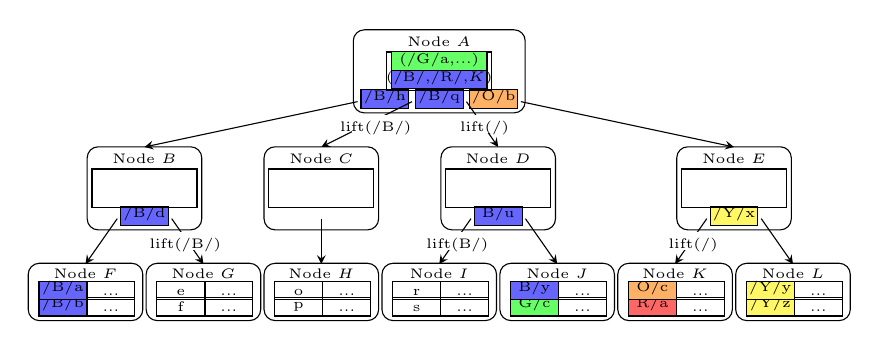
\begin{tikzpicture}[xscale=0.95, yscale=0.95]
            \node[anchor=south, rectangle, rounded corners, minimum height=.06\textwidth, minimum width=.12\textwidth, draw=black] at (0, 0) {};
            \node[anchor=south, font=\tiny] at (0, .036\textwidth) {Node $F$};
            \node[anchor=south, rectangle, minimum height=.015\textwidth, minimum width=.05\textwidth, draw=black, fill={blue!60}] at (-.025\textwidth, .005\textwidth) {};
            \node[anchor=south, font=\tiny] at (-.025\textwidth, 0) {/B/b};
            \node[anchor=south, rectangle, minimum height=.015\textwidth, minimum width=.05\textwidth, draw=black] at (.028\textwidth, .005\textwidth) {};
            \node[anchor=south, font=\tiny] at (.028\textwidth, 0) {...};
            \node[anchor=south, rectangle, minimum height=.015\textwidth, minimum width=.05\textwidth, draw=black, fill={blue!60}] at (-.025\textwidth, .023\textwidth) {};
            \node[anchor=south, font=\tiny] at (-.025\textwidth, .018\textwidth) {/B/a};
            \node[anchor=south, rectangle, minimum height=.015\textwidth, minimum width=.05\textwidth, draw=black] at (.028\textwidth, .023\textwidth) {};
            \node[anchor=south, font=\tiny] at (.028\textwidth, .018\textwidth) {...};

            \node[anchor=south, rectangle, rounded corners, minimum height=.06\textwidth, minimum width=.12\textwidth, draw=black] at (.13\textwidth, 0) {};
            \node[anchor=south, font=\tiny] at (.13\textwidth, .036\textwidth) {Node $G$};
            \node[anchor=south, rectangle, minimum height=.015\textwidth, minimum width=.05\textwidth, draw=black] at (.105\textwidth, .005\textwidth) {};
            \node[anchor=south, font=\tiny] at (.105\textwidth, 0) {f};
            \node[anchor=south, rectangle, minimum height=.015\textwidth, minimum width=.05\textwidth, draw=black] at (.158\textwidth, .005\textwidth) {};
            \node[anchor=south, font=\tiny] at (.158\textwidth, 0) {...};
            \node[anchor=south, rectangle, minimum height=.015\textwidth, minimum width=.05\textwidth, draw=black] at (.105\textwidth, .023\textwidth) {};
            \node[anchor=south, font=\tiny] at (.105\textwidth, .018\textwidth) {e};
            \node[anchor=south, rectangle, minimum height=.015\textwidth, minimum width=.05\textwidth, draw=black] at (.158\textwidth, .023\textwidth) {};
            \node[anchor=south, font=\tiny] at (.158\textwidth, .018\textwidth) {...};

            \node[anchor=south, rectangle, rounded corners, minimum height=.06\textwidth, minimum width=.12\textwidth, draw=black] at (.26\textwidth, 0) {};
            \node[anchor=south, font=\tiny] at (.26\textwidth, .036\textwidth) {Node $H$};
            \node[anchor=south, rectangle, minimum height=.015\textwidth, minimum width=.05\textwidth, draw=black] at (.235\textwidth, .005\textwidth) {};
            \node[anchor=south, font=\tiny] at (.235\textwidth, 0) {p};
            \node[anchor=south, rectangle, minimum height=.015\textwidth, minimum width=.05\textwidth, draw=black] at (.288\textwidth, .005\textwidth) {};
            \node[anchor=south, font=\tiny] at (.288\textwidth, 0) {...};
            \node[anchor=south, rectangle, minimum height=.015\textwidth, minimum width=.05\textwidth, draw=black] at (.235\textwidth, .023\textwidth) {};
            \node[anchor=south, font=\tiny] at (.235\textwidth, .018\textwidth) {o};
            \node[anchor=south, rectangle, minimum height=.015\textwidth, minimum width=.05\textwidth, draw=black] at (.288\textwidth, .023\textwidth) {};
            \node[anchor=south, font=\tiny] at (.288\textwidth, .018\textwidth) {...};

            \node[anchor=south, rectangle, rounded corners, minimum height=.06\textwidth, minimum width=.12\textwidth, draw=black] at (.39\textwidth, 0) {};
            \node[anchor=south, font=\tiny] at (.39\textwidth, .036\textwidth) {Node $I$};
            \node[anchor=south, rectangle, minimum height=.015\textwidth, minimum width=.05\textwidth, draw=black] at (.365\textwidth, .005\textwidth) {};
            \node[anchor=south, font=\tiny] at (.365\textwidth, 0) {s};
            \node[anchor=south, rectangle, minimum height=.015\textwidth, minimum width=.05\textwidth, draw=black] at (.418\textwidth, .005\textwidth) {};
            \node[anchor=south, font=\tiny] at (.418\textwidth, 0) {...};
            \node[anchor=south, rectangle, minimum height=.015\textwidth, minimum width=.05\textwidth, draw=black] at (.365\textwidth, .023\textwidth) {};
            \node[anchor=south, font=\tiny] at (.365\textwidth, .018\textwidth) {r};
            \node[anchor=south, rectangle, minimum height=.015\textwidth, minimum width=.05\textwidth, draw=black] at (.418\textwidth, .023\textwidth) {};
            \node[anchor=south, font=\tiny] at (.418\textwidth, .018\textwidth) {...};

            \node[anchor=south, rectangle, rounded corners, minimum height=.06\textwidth, minimum width=.12\textwidth, draw=black] at (.52\textwidth, 0) {};
            \node[anchor=south, font=\tiny] at (.52\textwidth, .036\textwidth) {Node $J$};
            \node[anchor=south, rectangle, minimum height=.015\textwidth, minimum width=.05\textwidth, draw=black, fill={green!60}] at (.495\textwidth, .005\textwidth) {};
            \node[anchor=south, font=\tiny] at (.495\textwidth, 0) {G/c};
            \node[anchor=south, rectangle, minimum height=.015\textwidth, minimum width=.05\textwidth, draw=black] at (.548\textwidth, .005\textwidth) {};
            \node[anchor=south, font=\tiny] at (.548\textwidth, 0) {...};
            \node[anchor=south, rectangle, minimum height=.015\textwidth, minimum width=.05\textwidth, draw=black, fill={blue!60}] at (.495\textwidth, .023\textwidth) {};
            \node[anchor=south, font=\tiny] at (.495\textwidth, .018\textwidth) {B/y};
            \node[anchor=south, rectangle, minimum height=.015\textwidth, minimum width=.05\textwidth, draw=black] at (.548\textwidth, .023\textwidth) {};
            \node[anchor=south, font=\tiny] at (.548\textwidth, .018\textwidth) {...};

            \node[anchor=south, rectangle, rounded corners, minimum height=.06\textwidth, minimum width=.12\textwidth, draw=black] at (.65\textwidth, 0) {};
            \node[anchor=south, font=\tiny] at (.65\textwidth, .036\textwidth) {Node $K$};
            \node[anchor=south, rectangle, minimum height=.015\textwidth, minimum width=.05\textwidth, draw=black, fill={red!60}] at (.625\textwidth, .005\textwidth) {};
            \node[anchor=south, font=\tiny] at (.625\textwidth, 0) {R/a};
            \node[anchor=south, rectangle, minimum height=.015\textwidth, minimum width=.05\textwidth, draw=black] at (.678\textwidth, .005\textwidth) {};
            \node[anchor=south, font=\tiny] at (.678\textwidth, 0) {...};
            \node[anchor=south, rectangle, minimum height=.015\textwidth, minimum width=.05\textwidth, draw=black, fill={orange!60}] at (.625\textwidth, .023\textwidth) {};
            \node[anchor=south, font=\tiny] at (.625\textwidth, .018\textwidth) {O/c};
            \node[anchor=south, rectangle, minimum height=.015\textwidth, minimum width=.05\textwidth, draw=black] at (.678\textwidth, .023\textwidth) {};
            \node[anchor=south, font=\tiny] at (.678\textwidth, .018\textwidth) {...};

            \node[anchor=south, rectangle, rounded corners, minimum height=.06\textwidth, minimum width=.12\textwidth, draw=black] at (.78\textwidth, 0) {};
            \node[anchor=south, font=\tiny] at (.78\textwidth, .036\textwidth) {Node $L$};
            \node[anchor=south, rectangle, minimum height=.015\textwidth, minimum width=.05\textwidth, draw=black, fill={yellow!60}] at (.755\textwidth, .005\textwidth) {};
            \node[anchor=south, font=\tiny] at (.755\textwidth, 0) {/Y/z};
            \node[anchor=south, rectangle, minimum height=.015\textwidth, minimum width=.05\textwidth, draw=black] at (.808\textwidth, .005\textwidth) {};
            \node[anchor=south, font=\tiny] at (.808\textwidth, 0) {...};
            \node[anchor=south, rectangle, minimum height=.015\textwidth, minimum width=.05\textwidth, draw=black, fill={yellow!60}] at (.755\textwidth, .023\textwidth) {};
            \node[anchor=south, font=\tiny] at (.755\textwidth, .018\textwidth) {/Y/y};
            \node[anchor=south, rectangle, minimum height=.015\textwidth, minimum width=.05\textwidth, draw=black] at (.808\textwidth, .023\textwidth) {};
            \node[anchor=south, font=\tiny] at (.808\textwidth, .018\textwidth) {...};

            \node[anchor=south, rectangle, rounded corners, minimum height=.087\textwidth, minimum width=.12\textwidth, draw=black] at (.065\textwidth, .1\textwidth) {};
            \node[anchor=south, font=\tiny] at (.065\textwidth, .163\textwidth) {Node $B$};
            \node[anchor=south, rectangle, minimum height=.015\textwidth, minimum width=.05\textwidth, draw=black, fill={blue!60}] at (.065\textwidth, .105\textwidth) {};
            \node[anchor=south, font=\tiny] at (.065\textwidth, .1\textwidth) {/B/d};
            \node[anchor=south, rectangle, minimum height=.04\textwidth, minimum width=.11\textwidth, draw=black] at (.065\textwidth, .125\textwidth) {};

            \node[anchor=south, rectangle, rounded corners, minimum height=.087\textwidth, minimum width=.12\textwidth, draw=black] at (.26\textwidth, .1\textwidth) {};
            \node[anchor=south, font=\tiny] at (.26\textwidth, .163\textwidth) {Node $C$};
            \node[anchor=south, rectangle, minimum height=.04\textwidth, minimum width=.11\textwidth, draw=black] at (.26\textwidth, .125\textwidth) {};

            \node[anchor=south, rectangle, rounded corners, minimum height=.087\textwidth, minimum width=.12\textwidth, draw=black] at (.455\textwidth, .1\textwidth) {};
            \node[anchor=south, font=\tiny] at (.455\textwidth, .163\textwidth) {Node $D$};
            \node[anchor=south, rectangle, minimum height=.015\textwidth, minimum width=.05\textwidth, draw=black, fill={blue!60}] at (.455\textwidth, .105\textwidth) {};
            \node[anchor=south, font=\tiny] at (.455\textwidth, .1\textwidth) {B/u};
            \node[anchor=south, rectangle, minimum height=.04\textwidth, minimum width=.11\textwidth, draw=black] at (.455\textwidth, .125\textwidth) {};

            \node[anchor=south, rectangle, rounded corners, minimum height=.087\textwidth, minimum width=.12\textwidth, draw=black] at (.715\textwidth, .1\textwidth) {};
            \node[anchor=south, font=\tiny] at (.715\textwidth, .163\textwidth) {Node $E$};
            \node[anchor=south, rectangle, minimum height=.015\textwidth, minimum width=.05\textwidth, draw=black, fill={yellow!60}] at (.715\textwidth, .105\textwidth) {};
            \node[anchor=south, font=\tiny] at (.715\textwidth, .1\textwidth) {/Y/x};
            \node[anchor=south, rectangle, minimum height=.04\textwidth, minimum width=.11\textwidth, draw=black] at (.715\textwidth, .125\textwidth) {};

            \node[anchor=south, rectangle, rounded corners, minimum height=.087\textwidth, minimum width=.18\textwidth, draw=black] at (.39\textwidth, .229\textwidth) {};
            \node[anchor=south, font=\tiny] at (.39\textwidth, .292\textwidth) {Node $A$};
            \node[anchor=south, rectangle, minimum height=.015\textwidth, minimum width=.05\textwidth, draw=black, fill={blue!60}] at (.33\textwidth, .234\textwidth) {};
            \node[anchor=south, font=\tiny] at (.33\textwidth, .229\textwidth) {/B/h};
            \node[anchor=south, rectangle, minimum height=.015\textwidth, minimum width=.05\textwidth, draw=black, fill={blue!60}] at (.39\textwidth, .234\textwidth) {};
            \node[anchor=south, font=\tiny] at (.39\textwidth, .229\textwidth) {/B/q};
            \node[anchor=south, rectangle, minimum height=.015\textwidth, minimum width=.05\textwidth, draw=black, fill={orange!60}] at (.45\textwidth, .234\textwidth) {};
            \node[anchor=south, font=\tiny] at (.45\textwidth, .229\textwidth) {/O/b};
            \node[anchor=south, rectangle, minimum height=.04\textwidth, minimum width=.11\textwidth, draw=black] at (.39\textwidth, .254\textwidth) {};
            \node[anchor=south, rectangle, minimum height=.015\textwidth, minimum width=.1\textwidth, draw=black, fill={blue!60}] at (.39\textwidth, .256\textwidth) {};
            \node[anchor=south, font=\tiny] at  (.39\textwidth, .25\textwidth) {\goto(/B/,/R/,$K$)};
            \node[anchor=south, rectangle, minimum height=.015\textwidth, minimum width=.1\textwidth, draw=black, fill={green!60}] at (.39\textwidth, .276\textwidth) {};
            \node[anchor=south, font=\tiny] at  (.39\textwidth, .27\textwidth) {\putm(/G/a,...)};

            \draw[->, >=stealth] (.035\textwidth, .113\textwidth) -- (0, .063\textwidth);
            \draw[->, >=stealth] (.095\textwidth, .113\textwidth) -- (.13\textwidth, .063\textwidth);
            \draw[->, >=stealth] (.26\textwidth, .113\textwidth) -- (.26\textwidth, .063\textwidth);
            \draw[->, >=stealth] (.425\textwidth, .113\textwidth) -- (.39\textwidth, .063\textwidth);
            \draw[->, >=stealth] (.485\textwidth, .113\textwidth) -- (.52\textwidth, .063\textwidth);
            \draw[->, >=stealth] (.685\textwidth, .113\textwidth) -- (.65\textwidth, .063\textwidth);
            \draw[->, >=stealth] (.745\textwidth, .113\textwidth) -- (.78\textwidth, .063\textwidth);
            \draw[->, >=stealth] (.3\textwidth, .242\textwidth) -- (.065\textwidth, .192\textwidth);
            \draw[->, >=stealth] (.36\textwidth, .242\textwidth) -- (.26\textwidth, .192\textwidth);
            \draw[->, >=stealth] (.42\textwidth, .242\textwidth) -- (.455\textwidth, .192\textwidth);
            \draw[->, >=stealth] (.48\textwidth, .242\textwidth) -- (.715\textwidth, .192\textwidth);

            \node[anchor=north,rectangle, minimum height=.015\textwidth, minimum width=.05\textwidth, fill={white}] at (.32\textwidth, .228\textwidth) {};
            \node[anchor=north, font=\tiny] at (.32\textwidth, .231\textwidth) {lift(/B/)};
            \node[anchor=north,rectangle, minimum height=.015\textwidth, minimum width=.05\textwidth, fill={white}] at (.44\textwidth, .228\textwidth) {};
            \node[anchor=north, font=\tiny] at (.44\textwidth, .231\textwidth) {lift(/)};
            \node[anchor=north,rectangle, minimum height=.015\textwidth, minimum width=.05\textwidth, fill={white}] at (.11\textwidth, .099\textwidth) {};
            \node[anchor=north, font=\tiny] at (.11\textwidth, .102\textwidth) {lift(/B/)};
            \node[anchor=north,rectangle, minimum height=.015\textwidth, minimum width=.05\textwidth, fill={white}] at (.41\textwidth, .099\textwidth) {};
            \node[anchor=north, font=\tiny] at (.41\textwidth, .102\textwidth) {lift(B/)};
            \node[anchor=north,rectangle, minimum height=.015\textwidth, minimum width=.05\textwidth, fill={white}] at (.67\textwidth, .099\textwidth) {};
            \node[anchor=north, font=\tiny] at (.67\textwidth, .102\textwidth) {lift(/)};
        \end{tikzpicture}
        \caption{\label{subfig:flush-1} The lifted \bedag wants to flush the
            \goto message from Node $A$, however, the \goto message doesn't
            fit into a single child.}
    \end{subfigure}
    \begin{subfigure}{\textwidth}
        \centering
        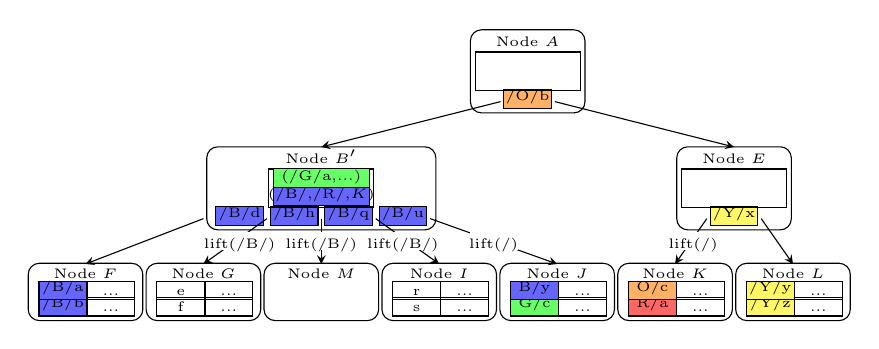
\begin{tikzpicture}[xscale=0.95, yscale=0.95]
            \node[anchor=south, rectangle, rounded corners, minimum height=.06\textwidth, minimum width=.12\textwidth, draw=black] at (0, 0) {};
            \node[anchor=south, font=\tiny] at (0, .036\textwidth) {Node $F$};
            \node[anchor=south, rectangle, minimum height=.015\textwidth, minimum width=.05\textwidth, draw=black, fill={blue!60}] at (-.025\textwidth, .005\textwidth) {};
            \node[anchor=south, font=\tiny] at (-.025\textwidth, 0) {/B/b};
            \node[anchor=south, rectangle, minimum height=.015\textwidth, minimum width=.05\textwidth, draw=black] at (.028\textwidth, .005\textwidth) {};
            \node[anchor=south, font=\tiny] at (.028\textwidth, 0) {...};
            \node[anchor=south, rectangle, minimum height=.015\textwidth, minimum width=.05\textwidth, draw=black, fill={blue!60}] at (-.025\textwidth, .023\textwidth) {};
            \node[anchor=south, font=\tiny] at (-.025\textwidth, .018\textwidth) {/B/a};
            \node[anchor=south, rectangle, minimum height=.015\textwidth, minimum width=.05\textwidth, draw=black] at (.028\textwidth, .023\textwidth) {};
            \node[anchor=south, font=\tiny] at (.028\textwidth, .018\textwidth) {...};

            \node[anchor=south, rectangle, rounded corners, minimum height=.06\textwidth, minimum width=.12\textwidth, draw=black] at (.13\textwidth, 0) {};
            \node[anchor=south, font=\tiny] at (.13\textwidth, .036\textwidth) {Node $G$};
            \node[anchor=south, rectangle, minimum height=.015\textwidth, minimum width=.05\textwidth, draw=black] at (.105\textwidth, .005\textwidth) {};
            \node[anchor=south, font=\tiny] at (.105\textwidth, 0) {f};
            \node[anchor=south, rectangle, minimum height=.015\textwidth, minimum width=.05\textwidth, draw=black] at (.158\textwidth, .005\textwidth) {};
            \node[anchor=south, font=\tiny] at (.158\textwidth, 0) {...};
            \node[anchor=south, rectangle, minimum height=.015\textwidth, minimum width=.05\textwidth, draw=black] at (.105\textwidth, .023\textwidth) {};
            \node[anchor=south, font=\tiny] at (.105\textwidth, .018\textwidth) {e};
            \node[anchor=south, rectangle, minimum height=.015\textwidth, minimum width=.05\textwidth, draw=black] at (.158\textwidth, .023\textwidth) {};
            \node[anchor=south, font=\tiny] at (.158\textwidth, .018\textwidth) {...};

            \node[anchor=south, rectangle, rounded corners, minimum height=.06\textwidth, minimum width=.12\textwidth, draw=black] at (.26\textwidth, 0) {};
            \node[anchor=south, font=\tiny] at (.26\textwidth, .036\textwidth) {Node $M$};

            \node[anchor=south, rectangle, rounded corners, minimum height=.06\textwidth, minimum width=.12\textwidth, draw=black] at (.39\textwidth, 0) {};
            \node[anchor=south, font=\tiny] at (.39\textwidth, .036\textwidth) {Node $I$};
            \node[anchor=south, rectangle, minimum height=.015\textwidth, minimum width=.05\textwidth, draw=black] at (.365\textwidth, .005\textwidth) {};
            \node[anchor=south, font=\tiny] at (.365\textwidth, 0) {s};
            \node[anchor=south, rectangle, minimum height=.015\textwidth, minimum width=.05\textwidth, draw=black] at (.418\textwidth, .005\textwidth) {};
            \node[anchor=south, font=\tiny] at (.418\textwidth, 0) {...};
            \node[anchor=south, rectangle, minimum height=.015\textwidth, minimum width=.05\textwidth, draw=black] at (.365\textwidth, .023\textwidth) {};
            \node[anchor=south, font=\tiny] at (.365\textwidth, .018\textwidth) {r};
            \node[anchor=south, rectangle, minimum height=.015\textwidth, minimum width=.05\textwidth, draw=black] at (.418\textwidth, .023\textwidth) {};
            \node[anchor=south, font=\tiny] at (.418\textwidth, .018\textwidth) {...};

            \node[anchor=south, rectangle, rounded corners, minimum height=.06\textwidth, minimum width=.12\textwidth, draw=black] at (.52\textwidth, 0) {};
            \node[anchor=south, font=\tiny] at (.52\textwidth, .036\textwidth) {Node $J$};
            \node[anchor=south, rectangle, minimum height=.015\textwidth, minimum width=.05\textwidth, draw=black, fill={green!60}] at (.495\textwidth, .005\textwidth) {};
            \node[anchor=south, font=\tiny] at (.495\textwidth, 0) {G/c};
            \node[anchor=south, rectangle, minimum height=.015\textwidth, minimum width=.05\textwidth, draw=black] at (.548\textwidth, .005\textwidth) {};
            \node[anchor=south, font=\tiny] at (.548\textwidth, 0) {...};
            \node[anchor=south, rectangle, minimum height=.015\textwidth, minimum width=.05\textwidth, draw=black, fill={blue!60}] at (.495\textwidth, .023\textwidth) {};
            \node[anchor=south, font=\tiny] at (.495\textwidth, .018\textwidth) {B/y};
            \node[anchor=south, rectangle, minimum height=.015\textwidth, minimum width=.05\textwidth, draw=black] at (.548\textwidth, .023\textwidth) {};
            \node[anchor=south, font=\tiny] at (.548\textwidth, .018\textwidth) {...};

            \node[anchor=south, rectangle, rounded corners, minimum height=.06\textwidth, minimum width=.12\textwidth, draw=black] at (.65\textwidth, 0) {};
            \node[anchor=south, font=\tiny] at (.65\textwidth, .036\textwidth) {Node $K$};
            \node[anchor=south, rectangle, minimum height=.015\textwidth, minimum width=.05\textwidth, draw=black, fill={red!60}] at (.625\textwidth, .005\textwidth) {};
            \node[anchor=south, font=\tiny] at (.625\textwidth, 0) {R/a};
            \node[anchor=south, rectangle, minimum height=.015\textwidth, minimum width=.05\textwidth, draw=black] at (.678\textwidth, .005\textwidth) {};
            \node[anchor=south, font=\tiny] at (.678\textwidth, 0) {...};
            \node[anchor=south, rectangle, minimum height=.015\textwidth, minimum width=.05\textwidth, draw=black, fill={orange!60}] at (.625\textwidth, .023\textwidth) {};
            \node[anchor=south, font=\tiny] at (.625\textwidth, .018\textwidth) {O/c};
            \node[anchor=south, rectangle, minimum height=.015\textwidth, minimum width=.05\textwidth, draw=black] at (.678\textwidth, .023\textwidth) {};
            \node[anchor=south, font=\tiny] at (.678\textwidth, .018\textwidth) {...};

            \node[anchor=south, rectangle, rounded corners, minimum height=.06\textwidth, minimum width=.12\textwidth, draw=black] at (.78\textwidth, 0) {};
            \node[anchor=south, font=\tiny] at (.78\textwidth, .036\textwidth) {Node $L$};
            \node[anchor=south, rectangle, minimum height=.015\textwidth, minimum width=.05\textwidth, draw=black, fill={yellow!60}] at (.755\textwidth, .005\textwidth) {};
            \node[anchor=south, font=\tiny] at (.755\textwidth, 0) {/Y/z};
            \node[anchor=south, rectangle, minimum height=.015\textwidth, minimum width=.05\textwidth, draw=black] at (.808\textwidth, .005\textwidth) {};
            \node[anchor=south, font=\tiny] at (.808\textwidth, 0) {...};
            \node[anchor=south, rectangle, minimum height=.015\textwidth, minimum width=.05\textwidth, draw=black, fill={yellow!60}] at (.755\textwidth, .023\textwidth) {};
            \node[anchor=south, font=\tiny] at (.755\textwidth, .018\textwidth) {/Y/y};
            \node[anchor=south, rectangle, minimum height=.015\textwidth, minimum width=.05\textwidth, draw=black] at (.808\textwidth, .023\textwidth) {};
            \node[anchor=south, font=\tiny] at (.808\textwidth, .018\textwidth) {...};

            \node[anchor=south, rectangle, rounded corners, minimum height=.087\textwidth, minimum width=.24\textwidth, draw=black] at (.26\textwidth, .1\textwidth) {};
            \node[anchor=south, font=\tiny] at (.26\textwidth, .163\textwidth) {Node $B'$};
            \node[anchor=south, rectangle, minimum height=.015\textwidth, minimum width=.05\textwidth, draw=black, fill={blue!60}] at (.17\textwidth, .105\textwidth) {};
            \node[anchor=south, font=\tiny] at (.17\textwidth, .1\textwidth) {/B/d};
            \node[anchor=south, rectangle, minimum height=.015\textwidth, minimum width=.05\textwidth, draw=black, fill={blue!60}] at (.23\textwidth, .105\textwidth) {};
            \node[anchor=south, font=\tiny] at (.23\textwidth, .1\textwidth) {/B/h};
            \node[anchor=south, rectangle, minimum height=.015\textwidth, minimum width=.05\textwidth, draw=black, fill={blue!60}] at (.29\textwidth, .105\textwidth) {};
            \node[anchor=south, font=\tiny] at (.29\textwidth, .1\textwidth) {/B/q};
            \node[anchor=south, rectangle, minimum height=.015\textwidth, minimum width=.05\textwidth, draw=black, fill={blue!60}] at (.35\textwidth, .105\textwidth) {};
            \node[anchor=south, font=\tiny] at (.35\textwidth, .1\textwidth) {/B/u};
            \node[anchor=south, rectangle, minimum height=.04\textwidth, minimum width=.11\textwidth, draw=black] at (.26\textwidth, .125\textwidth) {};
            \node[anchor=south, rectangle, minimum height=.015\textwidth, minimum width=.1\textwidth, draw=black, fill={blue!60}] at (.26\textwidth, .127\textwidth) {};
            \node[anchor=south, font=\tiny] at  (.26\textwidth, .121\textwidth) {\goto(/B/,/R/,$K$)};
            \node[anchor=south, rectangle, minimum height=.015\textwidth, minimum width=.1\textwidth, draw=black, fill={green!60}] at (.26\textwidth, .147\textwidth) {};
            \node[anchor=south, font=\tiny] at  (.26\textwidth, .141\textwidth) {\putm(/G/a,...)};

            \node[anchor=south, rectangle, rounded corners, minimum height=.087\textwidth, minimum width=.12\textwidth, draw=black] at (.715\textwidth, .1\textwidth) {};
            \node[anchor=south, font=\tiny] at (.715\textwidth, .163\textwidth) {Node $E$};
            \node[anchor=south, rectangle, minimum height=.015\textwidth, minimum width=.05\textwidth, draw=black, fill={yellow!60}] at (.715\textwidth, .105\textwidth) {};
            \node[anchor=south, font=\tiny] at (.715\textwidth, .1\textwidth) {/Y/x};
            \node[anchor=south, rectangle, minimum height=.04\textwidth, minimum width=.11\textwidth, draw=black] at (.715\textwidth, .125\textwidth) {};

            \node[anchor=south, rectangle, rounded corners, minimum height=.087\textwidth, minimum width=.12\textwidth, draw=black] at (.4875\textwidth, .229\textwidth) {};
            \node[anchor=south, font=\tiny] at (.4875\textwidth, .292\textwidth) {Node $A$};
            \node[anchor=south, rectangle, minimum height=.015\textwidth, minimum width=.05\textwidth, draw=black, fill={orange!60}] at (.4875\textwidth, .234\textwidth) {};
            \node[anchor=south, font=\tiny] at (.4875\textwidth, .229\textwidth) {/O/b};
            \node[anchor=south, rectangle, minimum height=.04\textwidth, minimum width=.11\textwidth, draw=black] at (.4875\textwidth, .254\textwidth) {};

            \draw[->, >=stealth] (.13\textwidth, .113\textwidth) -- (0, .063\textwidth);
            \draw[->, >=stealth] (.20\textwidth, .113\textwidth) -- (.13\textwidth, .063\textwidth);
            \draw[->, >=stealth] (.26\textwidth, .113\textwidth) -- (.26\textwidth, .063\textwidth);
            \draw[->, >=stealth] (.32\textwidth, .113\textwidth) -- (.39\textwidth, .063\textwidth);
            \draw[->, >=stealth] (.38\textwidth, .113\textwidth) -- (.52\textwidth, .063\textwidth);
            \draw[->, >=stealth] (.685\textwidth, .113\textwidth) -- (.65\textwidth, .063\textwidth);
            \draw[->, >=stealth] (.745\textwidth, .113\textwidth) -- (.78\textwidth, .063\textwidth);
            \draw[->, >=stealth] (.4575\textwidth, .242\textwidth) -- (.26\textwidth, .192\textwidth);
            \draw[->, >=stealth] (.5175\textwidth, .242\textwidth) -- (.715\textwidth, .192\textwidth);

            \node[anchor=north,rectangle, minimum height=.015\textwidth, minimum width=.05\textwidth, fill={white}] at (.17\textwidth, .099\textwidth) {};
            \node[anchor=north, font=\tiny] at (.17\textwidth, .102\textwidth) {lift(/B/)};
            \node[anchor=north,rectangle, minimum height=.015\textwidth, minimum width=.05\textwidth, fill={white}] at (.26\textwidth, .099\textwidth) {};
            \node[anchor=north, font=\tiny] at (.26\textwidth, .102\textwidth) {lift(/B/)};
            \node[anchor=north,rectangle, minimum height=.015\textwidth, minimum width=.05\textwidth, fill={white}] at (.35\textwidth, .099\textwidth) {};
            \node[anchor=north, font=\tiny] at (.35\textwidth, .102\textwidth) {lift(/B/)};
            \node[anchor=north,rectangle, minimum height=.015\textwidth, minimum width=.05\textwidth, fill={white}] at (.45\textwidth, .099\textwidth) {};
            \node[anchor=north, font=\tiny] at (.45\textwidth, .102\textwidth) {lift(/)};
            \node[anchor=north,rectangle, minimum height=.015\textwidth, minimum width=.05\textwidth, fill={white}] at (.67\textwidth, .099\textwidth) {};
            \node[anchor=north, font=\tiny] at (.67\textwidth, .102\textwidth) {lift(/)};
        \end{tikzpicture}
        \caption{\label{subfig:flush-2} The lifted \bedag garbage-collects Node
            $C$ and merges Node $B$ and $D$ into Node $B'$,
            which can accommodate the \goto message.}
    \end{subfigure}
    \caption[The \bedag merges children before flushing a \goto message]{\label{fig:flush}
        When a node tries to flush a \goto message, there may be more than
        one child that overlaps with the key range of the \goto message.
        In this case, the \bedag must merge children to create a single child
        that can accommodate the \goto message.}
\end{figure}


In the more complicated case, a \goto message can overlap with the key ranges
of multiple children.
There are at most two fringe children whose key ranges are partly covered by the
key range of the \goto message,
and partly out of the key range of the \goto message;
there are also some interior children whose key ranges are entirely
within the key range occluded by the \goto message.
The lift \bedag needs to create a single child that can accommodate the \goto
message.

To this end, the \bedag removes the references and pointers to the
interior children (potentially garbage-collecting these nodes, if this is
the last reference),
and merges the two fringe children into one child.
Removing interior children creates a key range that is not covered by the
fringe children.
One solution is to expand the key range of one fringe child,
however, changing the key range of a node means re-lifting the node and at
least one descendant at each height.
To avoid touching any descendant of the fringe children,
we add an empty subtree that covers the key range as the child of the merged
node.

Figure~\ref{fig:flush} shows an example of merging children before flushing a
\goto message.
In Figure~\ref{subfig:flush-1}, Node $B$, $C$ and $D$ all overlaps with the
range of the \goto message.
Node $B$ AND $D$ are fringe children, while Node $C$ is an interior child.
To flush the \goto message, in Figure~\ref{subfig:flush-2}, the lifted \bedag
garbage-collects Node $C$ and merges Node $B$ and $D$ into Node $B'$.
After the merge, Node $A$ flushes the \goto message to Node $B'$.
Note in the example, the merge creates an empty node, Node $M$, to cover the key
range (``/B/h'', ``/B/q'').

In special cases, there can be only one or no fringe child.
If there is only one fringe child, we removes the interior children and add
an empty subtree to cover the key range as one child of the fringe child.
If there is no fringe child, we remove the interior child and add an empty
subtree to cover the key range as the child of the node.

\paragraph{Converting \goto messages to pivots and parent-to-child pointers.}
After the merging process, there is only one child whose key range overlaps
with the key range of the \goto message.
If the child is higher than the source LCA of the \goto message,
we can simple flush the \goto message to the child buffer.
However, if the child is at the same height as the source LCA,
we cannot flush the \goto message.
Otherwise, the \goto message would redirect queries to a node at the same level,
which breaks the asymptotic I/O costs of queries.

In such scenarios, the \goto message is converted into into pivots and a
parent-to-child pointer in the node.

This is done by adding \dpre$_{min}$ and \dpre$_{max}$ as two new pivots and
set the parent-to-child pointer between the two pivots to the source LCA of the
\goto message.
Assume \dpre$_{min}$ and \dpre$_{max}$ are in the range of child $i$ of the node,
i.e., $\dpre_{min}, \dpre_{max} \in (pivot_{i},pivot_{i+1})$.
Adding \dpre$_{min}$ and \dpre$_{max}$ as two new pivots creates 3 key ranges,
$(pivot_{i},\dpre_{min})$, $(\dpre_{min},\dpre_{max})$ and
$(\dpre_{max}, pivot_{i+1})$.
Key range $(\dpre_{min},\dpre_{max})$ is cover in the source LCA of the \goto
message, while the other two are covered by child $i$.

However, all three parent-to-child pointers now points to a child whose key
range is different than those specified in the node.
In particular, child $i$ has range $(pivot_{i},pivot_{i+1})$ but bounded by
$(pivot_{i},\dpre_{min})$ or $(\dpre_{max}, pivot_{i+1})$.
The source LCA has a key range that might be larger than
$(\spre_{min}, \spre_{max})$ but bounded by $(\dpre_{min},\dpre_{max})$.
A smaller key range may lift a longer prefix through the parent-to-child
pointer.

The problem is solved by augmenting parent-to-child pointers with \xf functions,
which is the same as the \xf function described in \goto messages.
Each parent-to-child pointer now has a \xf function with a prefix.
After the query lifts its search key by the LCP of two pivots, the \xf function
prepends its prefix to the search key.
Also, \xf functions serves as filters, bounding the results queries may return.

\begin{figure}
    \begin{subfigure}{\textwidth}
        \centering
        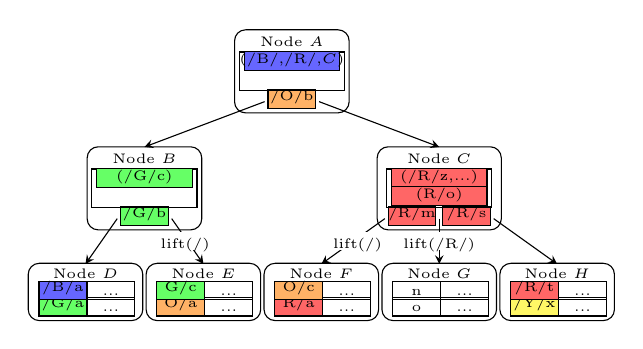
\begin{tikzpicture}[xscale=0.95, yscale=0.95]
            \node[anchor=south, rectangle, rounded corners, minimum height=.06\textwidth, minimum width=.12\textwidth, draw=black] at (0, 0) {};
            \node[anchor=south, font=\tiny] at (0, .036\textwidth) {Node $F$};
            \node[anchor=south, rectangle, minimum height=.015\textwidth, minimum width=.05\textwidth, draw=black, fill={red!60}] at (-.025\textwidth, .005\textwidth) {};
            \node[anchor=south, font=\tiny] at (-.025\textwidth, 0) {R/a};
            \node[anchor=south, rectangle, minimum height=.015\textwidth, minimum width=.05\textwidth, draw=black] at (.028\textwidth, .005\textwidth) {};
            \node[anchor=south, font=\tiny] at (.028\textwidth, 0) {...};
            \node[anchor=south, rectangle, minimum height=.015\textwidth, minimum width=.05\textwidth, draw=black, fill={orange!60}] at (-.025\textwidth, .023\textwidth) {};
            \node[anchor=south, font=\tiny] at (-.025\textwidth, .018\textwidth) {O/c};
            \node[anchor=south, rectangle, minimum height=.015\textwidth, minimum width=.05\textwidth, draw=black] at (.028\textwidth, .023\textwidth) {};
            \node[anchor=south, font=\tiny] at (.028\textwidth, .018\textwidth) {...};

            \node[anchor=south, rectangle, rounded corners, minimum height=.06\textwidth, minimum width=.12\textwidth, draw=black] at (.13\textwidth, 0) {};
            \node[anchor=south, font=\tiny] at (.13\textwidth, .036\textwidth) {Node $G$};
            \node[anchor=south, rectangle, minimum height=.015\textwidth, minimum width=.05\textwidth, draw=black] at (.105\textwidth, .005\textwidth) {};
            \node[anchor=south, font=\tiny] at (.105\textwidth, 0) {o};
            \node[anchor=south, rectangle, minimum height=.015\textwidth, minimum width=.05\textwidth, draw=black] at (.158\textwidth, .005\textwidth) {};
            \node[anchor=south, font=\tiny] at (.158\textwidth, 0) {...};
            \node[anchor=south, rectangle, minimum height=.015\textwidth, minimum width=.05\textwidth, draw=black] at (.105\textwidth, .023\textwidth) {};
            \node[anchor=south, font=\tiny] at (.105\textwidth, .018\textwidth) {n};
            \node[anchor=south, rectangle, minimum height=.015\textwidth, minimum width=.05\textwidth, draw=black] at (.158\textwidth, .023\textwidth) {};
            \node[anchor=south, font=\tiny] at (.158\textwidth, .018\textwidth) {...};

            \node[anchor=south, rectangle, rounded corners, minimum height=.06\textwidth, minimum width=.12\textwidth, draw=black] at (.26\textwidth, 0) {};
            \node[anchor=south, font=\tiny] at (.26\textwidth, .036\textwidth) {Node $H$};
            \node[anchor=south, rectangle, minimum height=.015\textwidth, minimum width=.05\textwidth, draw=black, fill={yellow!60}] at (.235\textwidth, .005\textwidth) {};
            \node[anchor=south, font=\tiny] at (.235\textwidth, 0) {/Y/x};
            \node[anchor=south, rectangle, minimum height=.015\textwidth, minimum width=.05\textwidth, draw=black] at (.288\textwidth, .005\textwidth) {};
            \node[anchor=south, font=\tiny] at (.288\textwidth, 0) {...};
            \node[anchor=south, rectangle, minimum height=.015\textwidth, minimum width=.05\textwidth, draw=black, fill={red!60}] at (.235\textwidth, .023\textwidth) {};
            \node[anchor=south, font=\tiny] at (.235\textwidth, .018\textwidth) {/R/t};
            \node[anchor=south, rectangle, minimum height=.015\textwidth, minimum width=.05\textwidth, draw=black] at (.288\textwidth, .023\textwidth) {};
            \node[anchor=south, font=\tiny] at (.288\textwidth, .018\textwidth) {...};

            \node[anchor=south, rectangle, rounded corners, minimum height=.06\textwidth, minimum width=.12\textwidth, draw=black] at (-.13\textwidth, 0) {};
            \node[anchor=south, font=\tiny] at (-.13\textwidth, .036\textwidth) {Node $E$};
            \node[anchor=south, rectangle, minimum height=.015\textwidth, minimum width=.05\textwidth, draw=black, fill={orange!60}] at (-.155\textwidth, .005\textwidth) {};
            \node[anchor=south, font=\tiny] at (-.155\textwidth, 0) {O/a};
            \node[anchor=south, rectangle, minimum height=.015\textwidth, minimum width=.05\textwidth, draw=black] at (-.102\textwidth, .005\textwidth) {};
            \node[anchor=south, font=\tiny] at (-.102\textwidth, 0) {...};
            \node[anchor=south, rectangle, minimum height=.015\textwidth, minimum width=.05\textwidth, draw=black, fill={green!60}] at (-.155\textwidth, .023\textwidth) {};
            \node[anchor=south, font=\tiny] at (-.155\textwidth, .018\textwidth) {G/c};
            \node[anchor=south, rectangle, minimum height=.015\textwidth, minimum width=.05\textwidth, draw=black] at (-.102\textwidth, .023\textwidth) {};
            \node[anchor=south, font=\tiny] at (-.102\textwidth, .018\textwidth) {...};

            \node[anchor=south, rectangle, rounded corners, minimum height=.06\textwidth, minimum width=.12\textwidth, draw=black] at (-.26\textwidth, 0) {};
            \node[anchor=south, font=\tiny] at (-.26\textwidth, .036\textwidth) {Node $D$};
            \node[anchor=south, rectangle, minimum height=.015\textwidth, minimum width=.05\textwidth, draw=black, fill={green!60}] at (-.285\textwidth, .005\textwidth) {};
            \node[anchor=south, font=\tiny] at (-.285\textwidth, 0) {/G/a};
            \node[anchor=south, rectangle, minimum height=.015\textwidth, minimum width=.05\textwidth, draw=black] at (-.232\textwidth, .005\textwidth) {};
            \node[anchor=south, font=\tiny] at (-.232\textwidth, 0) {...};
            \node[anchor=south, rectangle, minimum height=.015\textwidth, minimum width=.05\textwidth, draw=black, fill={blue!60}] at (-.285\textwidth, .023\textwidth) {};
            \node[anchor=south, font=\tiny] at (-.285\textwidth, .018\textwidth) {/B/a};
            \node[anchor=south, rectangle, minimum height=.015\textwidth, minimum width=.05\textwidth, draw=black] at (-.232\textwidth, .023\textwidth) {};
            \node[anchor=south, font=\tiny] at (-.232\textwidth, .018\textwidth) {...};

            \node[anchor=south, rectangle, rounded corners, minimum height=.087\textwidth, minimum width=.12\textwidth, draw=black] at (-.195\textwidth, .1\textwidth) {};
            \node[anchor=south, font=\tiny] at (-.195\textwidth, .163\textwidth) {Node $B$};
            \node[anchor=south, rectangle, minimum height=.015\textwidth, minimum width=.05\textwidth, draw=black, fill={green!60}] at (-.195\textwidth, .105\textwidth) {};
            \node[anchor=south, font=\tiny] at (-.195\textwidth, .1\textwidth) {/G/b};
            \node[anchor=south, rectangle, minimum height=.04\textwidth, minimum width=.11\textwidth, draw=black] at (-.195\textwidth, .125\textwidth) {};
            \node[anchor=south, rectangle, minimum height=.015\textwidth, minimum width=.1\textwidth, draw=black, fill={green!60}] at (-.195\textwidth, .147\textwidth) {};
            \node[anchor=south, font=\tiny] at  (-.195\textwidth, .141\textwidth) {\delm(/G/c)};

            \node[anchor=south, rectangle, rounded corners, minimum height=.087\textwidth, minimum width=.13\textwidth, draw=black] at (.13\textwidth, .1\textwidth) {};
            \node[anchor=south, font=\tiny] at (.13\textwidth, .163\textwidth) {Node $C$};
            \node[anchor=south, rectangle, minimum height=.015\textwidth, minimum width=.05\textwidth, draw=black, fill={red!60}] at (.1\textwidth, .105\textwidth) {};
            \node[anchor=south, font=\tiny] at (.1\textwidth, .1\textwidth) {/R/m};
            \node[anchor=south, rectangle, minimum height=.015\textwidth, minimum width=.05\textwidth, draw=black, fill={red!60}] at (.16\textwidth, .105\textwidth) {};
            \node[anchor=south, font=\tiny] at (.16\textwidth, .1\textwidth) {/R/s};
            \node[anchor=south, rectangle, minimum height=.04\textwidth, minimum width=.11\textwidth, draw=black] at (.13\textwidth, .125\textwidth) {};
            \node[anchor=south, rectangle, minimum height=.015\textwidth, minimum width=.1\textwidth, draw=black, fill={red!60}] at (.13\textwidth, .147\textwidth) {};
            \node[anchor=south, font=\tiny] at  (.13\textwidth, .141\textwidth) {\putm(/R/z,...)};
            \node[anchor=south, rectangle, minimum height=.015\textwidth, minimum width=.1\textwidth, draw=black, fill={red!60}] at (.13\textwidth, .127\textwidth) {};
            \node[anchor=south, font=\tiny] at  (.13\textwidth, .121\textwidth) {\delm(R/o)};

            \node[anchor=south, rectangle, rounded corners, minimum height=.087\textwidth, minimum width=.12\textwidth, draw=black] at (-.0325\textwidth, .229\textwidth) {};
            \node[anchor=south, font=\tiny] at (-.0325\textwidth, .292\textwidth) {Node $A$};
            \node[anchor=south, rectangle, minimum height=.015\textwidth, minimum width=.05\textwidth, draw=black, fill={orange!60}] at (-.0325\textwidth, .234\textwidth) {};
            \node[anchor=south, font=\tiny] at (-.0325\textwidth, .229\textwidth) {/O/b};
            \node[anchor=south, rectangle, minimum height=.04\textwidth, minimum width=.11\textwidth, draw=black] at (-.0325\textwidth, .254\textwidth) {};
            \node[anchor=south, rectangle, minimum height=.015\textwidth, minimum width=.1\textwidth, draw=black, fill={blue!60}] at (-.0325\textwidth, .276\textwidth) {};
            \node[anchor=south, font=\tiny] at  (-.0325\textwidth, .27\textwidth) {\goto(/B/,/R/,$C$)};

            \draw[->, >=stealth] (-.225\textwidth, .113\textwidth) -- (-.26\textwidth, .063\textwidth);
            \draw[->, >=stealth] (-.165\textwidth, .113\textwidth) -- (-.13\textwidth, .063\textwidth);
            \draw[->, >=stealth] (.13\textwidth, .113\textwidth) -- (.13\textwidth, .063\textwidth);
            \draw[->, >=stealth] (.19\textwidth, .113\textwidth) -- (.26\textwidth, .063\textwidth);
            \draw[->, >=stealth] (.07\textwidth, .113\textwidth) -- (0, .063\textwidth);
            \draw[->, >=stealth] (-.0625\textwidth, .242\textwidth) -- (-.195\textwidth, .192\textwidth);
            \draw[->, >=stealth] (-.0025\textwidth, .242\textwidth) -- (.13\textwidth, .192\textwidth);

            \node[anchor=north,rectangle, minimum height=.015\textwidth, minimum width=.05\textwidth, fill={white}] at (.13\textwidth, .099\textwidth) {};
            \node[anchor=north, font=\tiny] at (.13\textwidth, .102\textwidth) {lift(/R/)};
            \node[anchor=north,rectangle, minimum height=.015\textwidth, minimum width=.05\textwidth, fill={white}] at (.04\textwidth, .099\textwidth) {};
            \node[anchor=north, font=\tiny] at (.04\textwidth, .102\textwidth) {lift(/)};
            \node[anchor=north,rectangle, minimum height=.015\textwidth, minimum width=.05\textwidth, fill={white}] at (-.15\textwidth, .099\textwidth) {};
            \node[anchor=north, font=\tiny] at (-.15\textwidth, .102\textwidth) {lift(/)};
        \end{tikzpicture}
        \caption{\label{subfig:spvt-1} The \goto message cannot be flushed to
            Node $B$, which is at the same as Node $C$.}
    \end{subfigure}
    \begin{subfigure}{\textwidth}
        \centering
        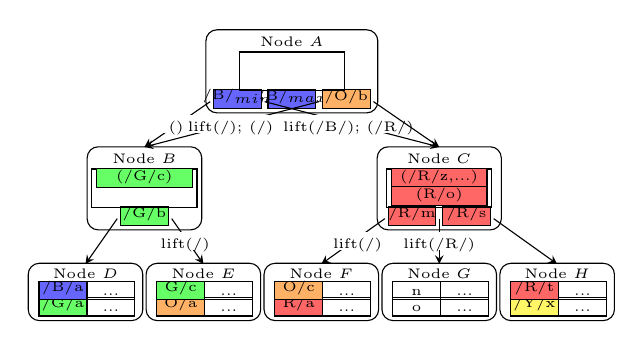
\begin{tikzpicture}[xscale=0.95, yscale=0.95]
            \node[anchor=south, rectangle, rounded corners, minimum height=.06\textwidth, minimum width=.12\textwidth, draw=black] at (0, 0) {};
            \node[anchor=south, font=\tiny] at (0, .036\textwidth) {Node $F$};
            \node[anchor=south, rectangle, minimum height=.015\textwidth, minimum width=.05\textwidth, draw=black, fill={red!60}] at (-.025\textwidth, .005\textwidth) {};
            \node[anchor=south, font=\tiny] at (-.025\textwidth, 0) {R/a};
            \node[anchor=south, rectangle, minimum height=.015\textwidth, minimum width=.05\textwidth, draw=black] at (.028\textwidth, .005\textwidth) {};
            \node[anchor=south, font=\tiny] at (.028\textwidth, 0) {...};
            \node[anchor=south, rectangle, minimum height=.015\textwidth, minimum width=.05\textwidth, draw=black, fill={orange!60}] at (-.025\textwidth, .023\textwidth) {};
            \node[anchor=south, font=\tiny] at (-.025\textwidth, .018\textwidth) {O/c};
            \node[anchor=south, rectangle, minimum height=.015\textwidth, minimum width=.05\textwidth, draw=black] at (.028\textwidth, .023\textwidth) {};
            \node[anchor=south, font=\tiny] at (.028\textwidth, .018\textwidth) {...};

            \node[anchor=south, rectangle, rounded corners, minimum height=.06\textwidth, minimum width=.12\textwidth, draw=black] at (.13\textwidth, 0) {};
            \node[anchor=south, font=\tiny] at (.13\textwidth, .036\textwidth) {Node $G$};
            \node[anchor=south, rectangle, minimum height=.015\textwidth, minimum width=.05\textwidth, draw=black] at (.105\textwidth, .005\textwidth) {};
            \node[anchor=south, font=\tiny] at (.105\textwidth, 0) {o};
            \node[anchor=south, rectangle, minimum height=.015\textwidth, minimum width=.05\textwidth, draw=black] at (.158\textwidth, .005\textwidth) {};
            \node[anchor=south, font=\tiny] at (.158\textwidth, 0) {...};
            \node[anchor=south, rectangle, minimum height=.015\textwidth, minimum width=.05\textwidth, draw=black] at (.105\textwidth, .023\textwidth) {};
            \node[anchor=south, font=\tiny] at (.105\textwidth, .018\textwidth) {n};
            \node[anchor=south, rectangle, minimum height=.015\textwidth, minimum width=.05\textwidth, draw=black] at (.158\textwidth, .023\textwidth) {};
            \node[anchor=south, font=\tiny] at (.158\textwidth, .018\textwidth) {...};

            \node[anchor=south, rectangle, rounded corners, minimum height=.06\textwidth, minimum width=.12\textwidth, draw=black] at (.26\textwidth, 0) {};
            \node[anchor=south, font=\tiny] at (.26\textwidth, .036\textwidth) {Node $H$};
            \node[anchor=south, rectangle, minimum height=.015\textwidth, minimum width=.05\textwidth, draw=black, fill={yellow!60}] at (.235\textwidth, .005\textwidth) {};
            \node[anchor=south, font=\tiny] at (.235\textwidth, 0) {/Y/x};
            \node[anchor=south, rectangle, minimum height=.015\textwidth, minimum width=.05\textwidth, draw=black] at (.288\textwidth, .005\textwidth) {};
            \node[anchor=south, font=\tiny] at (.288\textwidth, 0) {...};
            \node[anchor=south, rectangle, minimum height=.015\textwidth, minimum width=.05\textwidth, draw=black, fill={red!60}] at (.235\textwidth, .023\textwidth) {};
            \node[anchor=south, font=\tiny] at (.235\textwidth, .018\textwidth) {/R/t};
            \node[anchor=south, rectangle, minimum height=.015\textwidth, minimum width=.05\textwidth, draw=black] at (.288\textwidth, .023\textwidth) {};
            \node[anchor=south, font=\tiny] at (.288\textwidth, .018\textwidth) {...};

            \node[anchor=south, rectangle, rounded corners, minimum height=.06\textwidth, minimum width=.12\textwidth, draw=black] at (-.13\textwidth, 0) {};
            \node[anchor=south, font=\tiny] at (-.13\textwidth, .036\textwidth) {Node $E$};
            \node[anchor=south, rectangle, minimum height=.015\textwidth, minimum width=.05\textwidth, draw=black, fill={orange!60}] at (-.155\textwidth, .005\textwidth) {};
            \node[anchor=south, font=\tiny] at (-.155\textwidth, 0) {O/a};
            \node[anchor=south, rectangle, minimum height=.015\textwidth, minimum width=.05\textwidth, draw=black] at (-.102\textwidth, .005\textwidth) {};
            \node[anchor=south, font=\tiny] at (-.102\textwidth, 0) {...};
            \node[anchor=south, rectangle, minimum height=.015\textwidth, minimum width=.05\textwidth, draw=black, fill={green!60}] at (-.155\textwidth, .023\textwidth) {};
            \node[anchor=south, font=\tiny] at (-.155\textwidth, .018\textwidth) {G/c};
            \node[anchor=south, rectangle, minimum height=.015\textwidth, minimum width=.05\textwidth, draw=black] at (-.102\textwidth, .023\textwidth) {};
            \node[anchor=south, font=\tiny] at (-.102\textwidth, .018\textwidth) {...};

            \node[anchor=south, rectangle, rounded corners, minimum height=.06\textwidth, minimum width=.12\textwidth, draw=black] at (-.26\textwidth, 0) {};
            \node[anchor=south, font=\tiny] at (-.26\textwidth, .036\textwidth) {Node $D$};
            \node[anchor=south, rectangle, minimum height=.015\textwidth, minimum width=.05\textwidth, draw=black, fill={green!60}] at (-.285\textwidth, .005\textwidth) {};
            \node[anchor=south, font=\tiny] at (-.285\textwidth, 0) {/G/a};
            \node[anchor=south, rectangle, minimum height=.015\textwidth, minimum width=.05\textwidth, draw=black] at (-.232\textwidth, .005\textwidth) {};
            \node[anchor=south, font=\tiny] at (-.232\textwidth, 0) {...};
            \node[anchor=south, rectangle, minimum height=.015\textwidth, minimum width=.05\textwidth, draw=black, fill={blue!60}] at (-.285\textwidth, .023\textwidth) {};
            \node[anchor=south, font=\tiny] at (-.285\textwidth, .018\textwidth) {/B/a};
            \node[anchor=south, rectangle, minimum height=.015\textwidth, minimum width=.05\textwidth, draw=black] at (-.232\textwidth, .023\textwidth) {};
            \node[anchor=south, font=\tiny] at (-.232\textwidth, .018\textwidth) {...};

            \node[anchor=south, rectangle, rounded corners, minimum height=.087\textwidth, minimum width=.12\textwidth, draw=black] at (-.195\textwidth, .1\textwidth) {};
            \node[anchor=south, font=\tiny] at (-.195\textwidth, .163\textwidth) {Node $B$};
            \node[anchor=south, rectangle, minimum height=.015\textwidth, minimum width=.05\textwidth, draw=black, fill={green!60}] at (-.195\textwidth, .105\textwidth) {};
            \node[anchor=south, font=\tiny] at (-.195\textwidth, .1\textwidth) {/G/b};
            \node[anchor=south, rectangle, minimum height=.04\textwidth, minimum width=.11\textwidth, draw=black] at (-.195\textwidth, .125\textwidth) {};
            \node[anchor=south, rectangle, minimum height=.015\textwidth, minimum width=.1\textwidth, draw=black, fill={green!60}] at (-.195\textwidth, .147\textwidth) {};
            \node[anchor=south, font=\tiny] at  (-.195\textwidth, .141\textwidth) {\delm(/G/c)};

            \node[anchor=south, rectangle, rounded corners, minimum height=.087\textwidth, minimum width=.13\textwidth, draw=black] at (.13\textwidth, .1\textwidth) {};
            \node[anchor=south, font=\tiny] at (.13\textwidth, .163\textwidth) {Node $C$};
            \node[anchor=south, rectangle, minimum height=.015\textwidth, minimum width=.05\textwidth, draw=black, fill={red!60}] at (.1\textwidth, .105\textwidth) {};
            \node[anchor=south, font=\tiny] at (.1\textwidth, .1\textwidth) {/R/m};
            \node[anchor=south, rectangle, minimum height=.015\textwidth, minimum width=.05\textwidth, draw=black, fill={red!60}] at (.16\textwidth, .105\textwidth) {};
            \node[anchor=south, font=\tiny] at (.16\textwidth, .1\textwidth) {/R/s};
            \node[anchor=south, rectangle, minimum height=.04\textwidth, minimum width=.11\textwidth, draw=black] at (.13\textwidth, .125\textwidth) {};
            \node[anchor=south, rectangle, minimum height=.015\textwidth, minimum width=.1\textwidth, draw=black, fill={red!60}] at (.13\textwidth, .147\textwidth) {};
            \node[anchor=south, font=\tiny] at  (.13\textwidth, .141\textwidth) {\putm(/R/z,...)};
            \node[anchor=south, rectangle, minimum height=.015\textwidth, minimum width=.1\textwidth, draw=black, fill={red!60}] at (.13\textwidth, .127\textwidth) {};
            \node[anchor=south, font=\tiny] at  (.13\textwidth, .121\textwidth) {\delm(R/o)};

            \node[anchor=south, rectangle, rounded corners, minimum height=.087\textwidth, minimum width=.18\textwidth, draw=black] at (-.0325\textwidth, .229\textwidth) {};
            \node[anchor=south, font=\tiny] at (-.0325\textwidth, .292\textwidth) {Node $A$};
            \node[anchor=south, rectangle, minimum height=.015\textwidth, minimum width=.05\textwidth, draw=black, fill={blue!60}] at (-.0325\textwidth, .234\textwidth) {};
            \node[anchor=south, font=\tiny] at (-.0325\textwidth, .229\textwidth) {/B/$_{max}$};
            \node[anchor=south, rectangle, minimum height=.015\textwidth, minimum width=.05\textwidth, draw=black, fill={blue!60}] at (-.0925\textwidth, .234\textwidth) {};
            \node[anchor=south, font=\tiny] at (-.0925\textwidth, .229\textwidth) {/B/$_{min}$};
            \node[anchor=south, rectangle, minimum height=.015\textwidth, minimum width=.05\textwidth, draw=black, fill={orange!60}] at (.0275\textwidth, .234\textwidth) {};
            \node[anchor=south, font=\tiny] at (.0275\textwidth, .229\textwidth) {/O/b};
            \node[anchor=south, rectangle, minimum height=.04\textwidth, minimum width=.11\textwidth, draw=black] at (-.0325\textwidth, .254\textwidth) {};

            \draw[->, >=stealth] (-.225\textwidth, .113\textwidth) -- (-.26\textwidth, .063\textwidth);
            \draw[->, >=stealth] (-.165\textwidth, .113\textwidth) -- (-.13\textwidth, .063\textwidth);
            \draw[->, >=stealth] (.13\textwidth, .113\textwidth) -- (.13\textwidth, .063\textwidth);
            \draw[->, >=stealth] (.19\textwidth, .113\textwidth) -- (.26\textwidth, .063\textwidth);
            \draw[->, >=stealth] (.07\textwidth, .113\textwidth) -- (0, .063\textwidth);
            \draw[->, >=stealth] (-.1225\textwidth, .242\textwidth) -- (-.195\textwidth, .192\textwidth);
            \draw[->, >=stealth] (-.0625\textwidth, .242\textwidth) -- (.13\textwidth, .192\textwidth);
            \draw[->, >=stealth] (-.0025\textwidth, .242\textwidth) -- (-.195\textwidth, .192\textwidth);
            \draw[->, >=stealth] (.0575\textwidth, .242\textwidth) -- (.13\textwidth, .192\textwidth);

            \node[anchor=north,rectangle, minimum height=.015\textwidth, minimum width=.05\textwidth, fill={white}] at (.13\textwidth, .099\textwidth) {};
            \node[anchor=north, font=\tiny] at (.13\textwidth, .102\textwidth) {lift(/R/)};
            \node[anchor=north,rectangle, minimum height=.015\textwidth, minimum width=.05\textwidth, fill={white}] at (.04\textwidth, .099\textwidth) {};
            \node[anchor=north, font=\tiny] at (.04\textwidth, .102\textwidth) {lift(/)};
            \node[anchor=north,rectangle, minimum height=.015\textwidth, minimum width=.05\textwidth, fill={white}] at (-.15\textwidth, .099\textwidth) {};
            \node[anchor=north, font=\tiny] at (-.15\textwidth, .102\textwidth) {lift(/)};
            \node[anchor=north,rectangle, minimum height=.015\textwidth, minimum width=.05\textwidth, fill={white}] at (-.16\textwidth, .228\textwidth) {};
            \node[anchor=north, font=\tiny] at (-.16\textwidth, .231\textwidth) {\xf ()};
            \node[anchor=north,rectangle, minimum height=.015\textwidth, minimum width=.08\textwidth, fill={white}] at (-.1\textwidth, .228\textwidth) {};
            \node[anchor=north, font=\tiny] at (-.1\textwidth, .231\textwidth) {lift(/); \xf (/)};
            \node[anchor=north,rectangle, minimum height=.015\textwidth, minimum width=.08\textwidth, fill={white}] at (.03\textwidth, .228\textwidth) {};
            \node[anchor=north, font=\tiny] at (.03\textwidth, .231\textwidth) {lift(/B/); \xf (/R/)};
        \end{tikzpicture}
        \caption{\label{subfig:spvt-2} The \goto message becomes pivots and a
            parent-to-child pointer, and adds \xf functions to the parent-to-child pointers.}
    \end{subfigure}
    \caption[Transform a \goto message into pivots and a parent-to-child pointer]{\label{fig:spvt}
        When the lifted \bedag cannot flush a \goto message deeper, it
        transforms the \goto message into pivots and a parent-to-child pointers
        and adds \xf functions to the parent-to-child pointers.}
\end{figure}

Figure~\ref{fig:spvt} shows an example of the transformation.
The lifted \bedag cannot flush the \goto message from Node $A$ to Node $B$,
because Node $B$ is at the same height as its source LCA, Node $C$.
Therefore, it adds two pivots, ``/B/$_{min}$'' and ``/B/$_{max}$'', to Node $A$.
The parent-to-child pointer between ``/B/$_{min}$'' and ``/B/$_{max}$'' points
to the source LCA, Node $C$, and has a \xf function of ``/R/'', indicating a
key range mismatch and the additional prefix ``/R/'' for keys in the child.
Queries following that parent-to-child pointer should prepend prefix ``/R/''
after the normal lifting of ``/B/'' from its search key.
Also, they remember only keys between ``/R/$_{min}$'' and ``/R/$_{max}$'' in
the child are valid.
Similarly, two \xf functions are added to the other two pointers.
Note, for the leftmost pointer, though the \xf function contains no prefix,
it still serves as a filter for queries.

\paragraph{Fixing \xf functions in parent-to-child pointers.}
\goto messages adds \xf functions to parent-to-child pointers.
The \xf function transforms the search keys of queries by prepending its prefix
after normal key lifting through parent-to-child pointers.
Also, the \xf function indicates the child contains keys outside of the key range
specified by pivots in the parent and queries should ignore those keys following
the parent-to-child pointers.

The lifted \bedag resolves \xf functions through node flushes.
Specifically, when flushing from a parent to a child and the parent-to-child
pointer has a \xf function,
the lifted \bedag garbage-collects exterior children of the child whose key
ranges are completely outside of the key range specified by the pivots in parent.
Also, the lifted \bedag removes messages whose keys are outside of the key
range specified in the parent from the child buffer.
Then, for fringe children whose key ranges partly overlaps with that specified
in the parent, the \bedag propagates the \xf function to their parent-to-child
pointers.
At last, if the \xf function has a prefix, the \bedag lifts the prefix from
keys in the child.

\begin{figure}
    \begin{subfigure}{\textwidth}
        \centering
        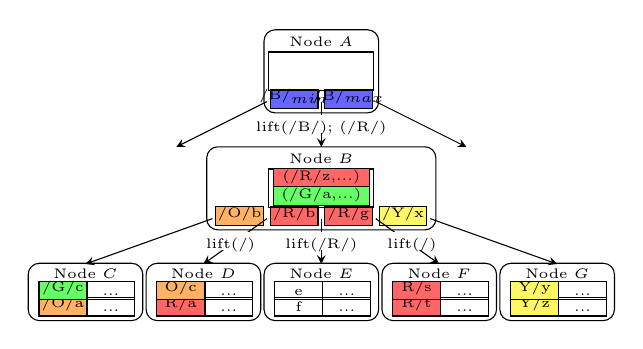
\begin{tikzpicture}[xscale=0.95, yscale=0.95]
            \node[anchor=south, rectangle, rounded corners, minimum height=.06\textwidth, minimum width=.12\textwidth, draw=black] at (0, 0) {};
            \node[anchor=south, font=\tiny] at (0, .036\textwidth) {Node $C$};
            \node[anchor=south, rectangle, minimum height=.015\textwidth, minimum width=.05\textwidth, draw=black, fill={orange!60}] at (-.025\textwidth, .005\textwidth) {};
            \node[anchor=south, font=\tiny] at (-.025\textwidth, 0) {/O/a};
            \node[anchor=south, rectangle, minimum height=.015\textwidth, minimum width=.05\textwidth, draw=black] at (.028\textwidth, .005\textwidth) {};
            \node[anchor=south, font=\tiny] at (.028\textwidth, 0) {...};
            \node[anchor=south, rectangle, minimum height=.015\textwidth, minimum width=.05\textwidth, draw=black, fill={green!60}] at (-.025\textwidth, .023\textwidth) {};
            \node[anchor=south, font=\tiny] at (-.025\textwidth, .018\textwidth) {/G/c};
            \node[anchor=south, rectangle, minimum height=.015\textwidth, minimum width=.05\textwidth, draw=black] at (.028\textwidth, .023\textwidth) {};
            \node[anchor=south, font=\tiny] at (.028\textwidth, .018\textwidth) {...};

            \node[anchor=south, rectangle, rounded corners, minimum height=.06\textwidth, minimum width=.12\textwidth, draw=black] at (.13\textwidth, 0) {};
            \node[anchor=south, font=\tiny] at (.13\textwidth, .036\textwidth) {Node $D$};
            \node[anchor=south, rectangle, minimum height=.015\textwidth, minimum width=.05\textwidth, draw=black, fill={red!60}] at (.105\textwidth, .005\textwidth) {};
            \node[anchor=south, font=\tiny] at (.105\textwidth, 0) {R/a};
            \node[anchor=south, rectangle, minimum height=.015\textwidth, minimum width=.05\textwidth, draw=black] at (.158\textwidth, .005\textwidth) {};
            \node[anchor=south, font=\tiny] at (.158\textwidth, 0) {...};
            \node[anchor=south, rectangle, minimum height=.015\textwidth, minimum width=.05\textwidth, draw=black, fill={orange!60}] at (.105\textwidth, .023\textwidth) {};
            \node[anchor=south, font=\tiny] at (.105\textwidth, .018\textwidth) {O/c};
            \node[anchor=south, rectangle, minimum height=.015\textwidth, minimum width=.05\textwidth, draw=black] at (.158\textwidth, .023\textwidth) {};
            \node[anchor=south, font=\tiny] at (.158\textwidth, .018\textwidth) {...};

            \node[anchor=south, rectangle, rounded corners, minimum height=.06\textwidth, minimum width=.12\textwidth, draw=black] at (.26\textwidth, 0) {};
            \node[anchor=south, font=\tiny] at (.26\textwidth, .036\textwidth) {Node $E$};
            \node[anchor=south, rectangle, minimum height=.015\textwidth, minimum width=.05\textwidth, draw=black] at (.235\textwidth, .005\textwidth) {};
            \node[anchor=south, font=\tiny] at (.235\textwidth, 0) {f};
            \node[anchor=south, rectangle, minimum height=.015\textwidth, minimum width=.05\textwidth, draw=black] at (.288\textwidth, .005\textwidth) {};
            \node[anchor=south, font=\tiny] at (.288\textwidth, 0) {...};
            \node[anchor=south, rectangle, minimum height=.015\textwidth, minimum width=.05\textwidth, draw=black] at (.235\textwidth, .023\textwidth) {};
            \node[anchor=south, font=\tiny] at (.235\textwidth, .018\textwidth) {e};
            \node[anchor=south, rectangle, minimum height=.015\textwidth, minimum width=.05\textwidth, draw=black] at (.288\textwidth, .023\textwidth) {};
            \node[anchor=south, font=\tiny] at (.288\textwidth, .018\textwidth) {...};

            \node[anchor=south, rectangle, rounded corners, minimum height=.06\textwidth, minimum width=.12\textwidth, draw=black] at (.39\textwidth, 0) {};
            \node[anchor=south, font=\tiny] at (.39\textwidth, .036\textwidth) {Node $F$};
            \node[anchor=south, rectangle, minimum height=.015\textwidth, minimum width=.05\textwidth, draw=black, fill={red!60}] at (.365\textwidth, .005\textwidth) {};
            \node[anchor=south, font=\tiny] at (.365\textwidth, 0) {R/t};
            \node[anchor=south, rectangle, minimum height=.015\textwidth, minimum width=.05\textwidth, draw=black] at (.418\textwidth, .005\textwidth) {};
            \node[anchor=south, font=\tiny] at (.418\textwidth, 0) {...};
            \node[anchor=south, rectangle, minimum height=.015\textwidth, minimum width=.05\textwidth, draw=black, fill={red!60}] at (.365\textwidth, .023\textwidth) {};
            \node[anchor=south, font=\tiny] at (.365\textwidth, .018\textwidth) {R/s};
            \node[anchor=south, rectangle, minimum height=.015\textwidth, minimum width=.05\textwidth, draw=black] at (.418\textwidth, .023\textwidth) {};
            \node[anchor=south, font=\tiny] at (.418\textwidth, .018\textwidth) {...};

            \node[anchor=south, rectangle, rounded corners, minimum height=.06\textwidth, minimum width=.12\textwidth, draw=black] at (.52\textwidth, 0) {};
            \node[anchor=south, font=\tiny] at (.52\textwidth, .036\textwidth) {Node $G$};
            \node[anchor=south, rectangle, minimum height=.015\textwidth, minimum width=.05\textwidth, draw=black, fill={yellow!60}] at (.495\textwidth, .005\textwidth) {};
            \node[anchor=south, font=\tiny] at (.495\textwidth, 0) {Y/z};
            \node[anchor=south, rectangle, minimum height=.015\textwidth, minimum width=.05\textwidth, draw=black] at (.548\textwidth, .005\textwidth) {};
            \node[anchor=south, font=\tiny] at (.548\textwidth, 0) {...};
            \node[anchor=south, rectangle, minimum height=.015\textwidth, minimum width=.05\textwidth, draw=black, fill={yellow!60}] at (.495\textwidth, .023\textwidth) {};
            \node[anchor=south, font=\tiny] at (.495\textwidth, .018\textwidth) {Y/y};
            \node[anchor=south, rectangle, minimum height=.015\textwidth, minimum width=.05\textwidth, draw=black] at (.548\textwidth, .023\textwidth) {};
            \node[anchor=south, font=\tiny] at (.548\textwidth, .018\textwidth) {...};

            \node[anchor=south, rectangle, rounded corners, minimum height=.087\textwidth, minimum width=.24\textwidth, draw=black] at (.26\textwidth, .1\textwidth) {};
            \node[anchor=south, font=\tiny] at (.26\textwidth, .163\textwidth) {Node $B$};
            \node[anchor=south, rectangle, minimum height=.015\textwidth, minimum width=.05\textwidth, draw=black, fill={orange!60}] at (.17\textwidth, .105\textwidth) {};
            \node[anchor=south, font=\tiny] at (.17\textwidth, .1\textwidth) {/O/b};
            \node[anchor=south, rectangle, minimum height=.015\textwidth, minimum width=.05\textwidth, draw=black, fill={red!60}] at (.23\textwidth, .105\textwidth) {};
            \node[anchor=south, font=\tiny] at (.23\textwidth, .1\textwidth) {/R/b};
            \node[anchor=south, rectangle, minimum height=.015\textwidth, minimum width=.05\textwidth, draw=black, fill={red!60}] at (.29\textwidth, .105\textwidth) {};
            \node[anchor=south, font=\tiny] at (.29\textwidth, .1\textwidth) {/R/g};
            \node[anchor=south, rectangle, minimum height=.015\textwidth, minimum width=.05\textwidth, draw=black, fill={yellow!60}] at (.35\textwidth, .105\textwidth) {};
            \node[anchor=south, font=\tiny] at (.35\textwidth, .1\textwidth) {/Y/x};
            \node[anchor=south, rectangle, minimum height=.04\textwidth, minimum width=.11\textwidth, draw=black] at (.26\textwidth, .125\textwidth) {};
            \node[anchor=south, rectangle, minimum height=.015\textwidth, minimum width=.1\textwidth, draw=black, fill={red!60}] at (.26\textwidth, .147\textwidth) {};
            \node[anchor=south, font=\tiny] at  (.26\textwidth, .141\textwidth) {\putm(/R/z,...)};
            \node[anchor=south, rectangle, minimum height=.015\textwidth, minimum width=.1\textwidth, draw=black, fill={green!60}] at (.26\textwidth, .127\textwidth) {};
            \node[anchor=south, font=\tiny] at  (.26\textwidth, .121\textwidth) {\putm(/G/a,...)};

            \node[anchor=south, rectangle, rounded corners, minimum height=.087\textwidth, minimum width=.12\textwidth, draw=black] at (.26\textwidth, .229\textwidth) {};
            \node[anchor=south, font=\tiny] at (.26\textwidth, .292\textwidth) {Node $A$};
            \node[anchor=south, rectangle, minimum height=.015\textwidth, minimum width=.05\textwidth, draw=black, fill={blue!60}] at (.23\textwidth, .234\textwidth) {};
            \node[anchor=south, font=\tiny] at (.23\textwidth, .229\textwidth) {/B/$_{min}$};
            \node[anchor=south, rectangle, minimum height=.015\textwidth, minimum width=.05\textwidth, draw=black, fill={blue!60}] at (.29\textwidth, .234\textwidth) {};
            \node[anchor=south, font=\tiny] at (.29\textwidth, .229\textwidth) {/B/$_{max}$};
            \node[anchor=south, rectangle, minimum height=.04\textwidth, minimum width=.11\textwidth, draw=black] at (.26\textwidth, .254\textwidth) {};

            \draw[->, >=stealth] (.14\textwidth, .113\textwidth) -- (0, .063\textwidth);
            \draw[->, >=stealth] (.20\textwidth, .113\textwidth) -- (.13\textwidth, .063\textwidth);
            \draw[->, >=stealth] (.26\textwidth, .113\textwidth) -- (.26\textwidth, .063\textwidth);
            \draw[->, >=stealth] (.32\textwidth, .113\textwidth) -- (.39\textwidth, .063\textwidth);
            \draw[->, >=stealth] (.38\textwidth, .113\textwidth) -- (.52\textwidth, .063\textwidth);
            \draw[->, >=stealth] (.26\textwidth, .242\textwidth) -- (.26\textwidth, .192\textwidth);
            \draw[->, >=stealth] (.20\textwidth, .242\textwidth) -- (.10\textwidth, .192\textwidth);
            \draw[->, >=stealth] (.32\textwidth, .242\textwidth) -- (.42\textwidth, .192\textwidth);

            \node[anchor=north,rectangle, minimum height=.015\textwidth, minimum width=.05\textwidth, fill={white}] at (.16\textwidth, .099\textwidth) {};
            \node[anchor=north, font=\tiny] at (.16\textwidth, .102\textwidth) {lift(/)};
            \node[anchor=north,rectangle, minimum height=.015\textwidth, minimum width=.05\textwidth, fill={white}] at (.26\textwidth, .099\textwidth) {};
            \node[anchor=north, font=\tiny] at (.26\textwidth, .102\textwidth) {lift(/R/)};
            \node[anchor=north,rectangle, minimum height=.015\textwidth, minimum width=.05\textwidth, fill={white}] at (.36\textwidth, .099\textwidth) {};
            \node[anchor=north, font=\tiny] at (.36\textwidth, .102\textwidth) {lift(/)};
            \node[anchor=north,rectangle, minimum height=.015\textwidth, minimum width=.08\textwidth, fill={white}] at (.26\textwidth, .228\textwidth) {};
            \node[anchor=north, font=\tiny] at (.26\textwidth, .231\textwidth) {lift(/B/); \xf (/R/)};
        \end{tikzpicture}
        \caption{\label{subfig:xf-1} The parent-to-child pointer from Node $A$
            to Node $B$ has \xf(``/R/'').}
    \end{subfigure}
    \begin{subfigure}{\textwidth}
        \centering
        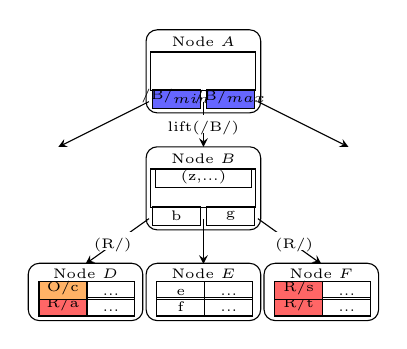
\begin{tikzpicture}[xscale=0.95, yscale=0.95]
            \node[anchor=south, rectangle, rounded corners, minimum height=.06\textwidth, minimum width=.12\textwidth, draw=black] at (.13\textwidth, 0) {};
            \node[anchor=south, font=\tiny] at (.13\textwidth, .036\textwidth) {Node $D$};
            \node[anchor=south, rectangle, minimum height=.015\textwidth, minimum width=.05\textwidth, draw=black, fill={red!60}] at (.105\textwidth, .005\textwidth) {};
            \node[anchor=south, font=\tiny] at (.105\textwidth, 0) {R/a};
            \node[anchor=south, rectangle, minimum height=.015\textwidth, minimum width=.05\textwidth, draw=black] at (.158\textwidth, .005\textwidth) {};
            \node[anchor=south, font=\tiny] at (.158\textwidth, 0) {...};
            \node[anchor=south, rectangle, minimum height=.015\textwidth, minimum width=.05\textwidth, draw=black, fill={orange!60}] at (.105\textwidth, .023\textwidth) {};
            \node[anchor=south, font=\tiny] at (.105\textwidth, .018\textwidth) {O/c};
            \node[anchor=south, rectangle, minimum height=.015\textwidth, minimum width=.05\textwidth, draw=black] at (.158\textwidth, .023\textwidth) {};
            \node[anchor=south, font=\tiny] at (.158\textwidth, .018\textwidth) {...};

            \node[anchor=south, rectangle, rounded corners, minimum height=.06\textwidth, minimum width=.12\textwidth, draw=black] at (.26\textwidth, 0) {};
            \node[anchor=south, font=\tiny] at (.26\textwidth, .036\textwidth) {Node $E$};
            \node[anchor=south, rectangle, minimum height=.015\textwidth, minimum width=.05\textwidth, draw=black] at (.235\textwidth, .005\textwidth) {};
            \node[anchor=south, font=\tiny] at (.235\textwidth, 0) {f};
            \node[anchor=south, rectangle, minimum height=.015\textwidth, minimum width=.05\textwidth, draw=black] at (.288\textwidth, .005\textwidth) {};
            \node[anchor=south, font=\tiny] at (.288\textwidth, 0) {...};
            \node[anchor=south, rectangle, minimum height=.015\textwidth, minimum width=.05\textwidth, draw=black] at (.235\textwidth, .023\textwidth) {};
            \node[anchor=south, font=\tiny] at (.235\textwidth, .018\textwidth) {e};
            \node[anchor=south, rectangle, minimum height=.015\textwidth, minimum width=.05\textwidth, draw=black] at (.288\textwidth, .023\textwidth) {};
            \node[anchor=south, font=\tiny] at (.288\textwidth, .018\textwidth) {...};

            \node[anchor=south, rectangle, rounded corners, minimum height=.06\textwidth, minimum width=.12\textwidth, draw=black] at (.39\textwidth, 0) {};
            \node[anchor=south, font=\tiny] at (.39\textwidth, .036\textwidth) {Node $F$};
            \node[anchor=south, rectangle, minimum height=.015\textwidth, minimum width=.05\textwidth, draw=black, fill={red!60}] at (.365\textwidth, .005\textwidth) {};
            \node[anchor=south, font=\tiny] at (.365\textwidth, 0) {R/t};
            \node[anchor=south, rectangle, minimum height=.015\textwidth, minimum width=.05\textwidth, draw=black] at (.418\textwidth, .005\textwidth) {};
            \node[anchor=south, font=\tiny] at (.418\textwidth, 0) {...};
            \node[anchor=south, rectangle, minimum height=.015\textwidth, minimum width=.05\textwidth, draw=black, fill={red!60}] at (.365\textwidth, .023\textwidth) {};
            \node[anchor=south, font=\tiny] at (.365\textwidth, .018\textwidth) {R/s};
            \node[anchor=south, rectangle, minimum height=.015\textwidth, minimum width=.05\textwidth, draw=black] at (.418\textwidth, .023\textwidth) {};
            \node[anchor=south, font=\tiny] at (.418\textwidth, .018\textwidth) {...};

            \node[anchor=south, rectangle, rounded corners, minimum height=.087\textwidth, minimum width=.12\textwidth, draw=black] at (.26\textwidth, .1\textwidth) {};
            \node[anchor=south, font=\tiny] at (.26\textwidth, .163\textwidth) {Node $B$};
            \node[anchor=south, rectangle, minimum height=.015\textwidth, minimum width=.05\textwidth, draw=black] at (.23\textwidth, .105\textwidth) {};
            \node[anchor=south, font=\tiny] at (.23\textwidth, .1\textwidth) {b};
            \node[anchor=south, rectangle, minimum height=.015\textwidth, minimum width=.05\textwidth, draw=black] at (.29\textwidth, .105\textwidth) {};
            \node[anchor=south, font=\tiny] at (.29\textwidth, .1\textwidth) {g};
            \node[anchor=south, rectangle, minimum height=.04\textwidth, minimum width=.11\textwidth, draw=black] at (.26\textwidth, .125\textwidth) {};
            \node[anchor=south, rectangle, minimum height=.015\textwidth, minimum width=.1\textwidth, draw=black] at (.26\textwidth, .147\textwidth) {};
            \node[anchor=south, font=\tiny] at  (.26\textwidth, .141\textwidth) {\putm(z,...)};

            \node[anchor=south, rectangle, rounded corners, minimum height=.087\textwidth, minimum width=.12\textwidth, draw=black] at (.26\textwidth, .229\textwidth) {};
            \node[anchor=south, font=\tiny] at (.26\textwidth, .292\textwidth) {Node $A$};
            \node[anchor=south, rectangle, minimum height=.015\textwidth, minimum width=.05\textwidth, draw=black, fill={blue!60}] at (.23\textwidth, .234\textwidth) {};
            \node[anchor=south, font=\tiny] at (.23\textwidth, .229\textwidth) {/B/$_{min}$};
            \node[anchor=south, rectangle, minimum height=.015\textwidth, minimum width=.05\textwidth, draw=black, fill={blue!60}] at (.29\textwidth, .234\textwidth) {};
            \node[anchor=south, font=\tiny] at (.29\textwidth, .229\textwidth) {/B/$_{max}$};
            \node[anchor=south, rectangle, minimum height=.04\textwidth, minimum width=.11\textwidth, draw=black] at (.26\textwidth, .254\textwidth) {};

            \draw[->, >=stealth] (.20\textwidth, .113\textwidth) -- (.13\textwidth, .063\textwidth);
            \draw[->, >=stealth] (.26\textwidth, .113\textwidth) -- (.26\textwidth, .063\textwidth);
            \draw[->, >=stealth] (.32\textwidth, .113\textwidth) -- (.39\textwidth, .063\textwidth);
            \draw[->, >=stealth] (.26\textwidth, .242\textwidth) -- (.26\textwidth, .192\textwidth);
            \draw[->, >=stealth] (.20\textwidth, .242\textwidth) -- (.10\textwidth, .192\textwidth);
            \draw[->, >=stealth] (.32\textwidth, .242\textwidth) -- (.42\textwidth, .192\textwidth);

            \node[anchor=north,rectangle, minimum height=.015\textwidth, minimum width=.05\textwidth, fill={white}] at (.16\textwidth, .099\textwidth) {};
            \node[anchor=north, font=\tiny] at (.16\textwidth, .102\textwidth) {\xf (R/)};
            \node[anchor=north,rectangle, minimum height=.015\textwidth, minimum width=.05\textwidth, fill={white}] at (.36\textwidth, .099\textwidth) {};
            \node[anchor=north, font=\tiny] at (.36\textwidth, .102\textwidth) {\xf (R/)};
            \node[anchor=north,rectangle, minimum height=.015\textwidth, minimum width=.08\textwidth, fill={white}] at (.26\textwidth, .228\textwidth) {};
            \node[anchor=north, font=\tiny] at (.26\textwidth, .231\textwidth) {lift(/B/)};
        \end{tikzpicture}
        \caption{\label{subfig:xf-2} To remove the \xf function, it discards
            exterior children and adds \xf functions to parent-to-child pointers
            of fringe children.}
    \end{subfigure}
    \caption[Resolving \xf functions in node flushes]{\label{fig:xf}
        During node flushes, the lifted \bedag resolves the \xf
        function associated with the parent-to-child pointer.}
\end{figure}

Figure~\ref{fig:xf} shows an example of fixing \xf functions in node flushes.
In Figure~\ref{subfig:xf-1}, the parent-to-child pointer from Node $A$ to
Node $B$ has a \xf function, \xf(``/R/'').
The key range specified by Node $A$ is (``/B/$_{min}$'',``/B/$_{max}$''), which
translates to (``/R/$_{min}$'',``/R/$_{max}$'') in Node $B$.
In Figure~\ref{subfig:xf-2}, the lifted \bedag garbage-collects exterior nodes,
Node $C$ and $G$
and adds \xf functions to pointers to fringe nodes, Node $D$ and $F$.
Also, it updates keys in Node $B$ by removing the prefix, ``/R/'',
in the \xf function.
Note, the message \putm(/G/a,...) is also removed from Node $B$
because it is out of the key range specified in Node $A$.

\section{Implementation}
\label{sec:rcimp}

\subsection{Preferential splitting}

Most of the work in range-clone and range-rename is about splitting fringe
nodes, separating keys with a prefix and keys without the prefix.
If all nodes are either interior nodes or exterior nodes, much less work is
needed.
Therefore, it is beneficial to reduce the number of fringe nodes.

The baseline \bet splits leaf nodes evenly.
When a leaf node needs to be split, the middle key in the leaf is picked as the
new pivot that separates the two new leaves.

Preferential splitting generates pivots that are potential splitting keys in
file system renames and maximize the common prefix under the leaf,
subject to the constraint that both leaves should be at least 1/4 full.
This strategy reduces the likelihood of having fringe nodes
in range-clone and bounds how unbalanced leaves can be.

A naive approach would compare all keys in the range of [1/4, 3/4] of the leaf
node and pick the pair of two adjacent keys that share the shortest common
prefix.
But this scan can be costly.
For example, in \betrfs, a full leaf node is 4 MiB in size and each key/value pair in
\texttt{meta\_db} is less than 200 Bytes, which means more than 10000 key
comparisons are required in this naive preferential splitting.

In fact, we can do preferential splitting that only requires the reading of two keys.
Because the shortest common prefix of adjacent keys is the same as the common
prefix of the smallest (at 1/4 of the leaf) candidate key, $k_{s}$, and
the largest (at 3/4 of the leaf) candidate key, $k_{l}$,
a good pivot can be constructed from these two keys.
In particular, preferential splitting generates a pivot that is the maximum key
with prefix $p_{s}$, where $p_{s}$ is the shortest prefix of $k_{s}$ that
contains the LCP of $k_{s}$ and $k_{l}$ and has a slash or a end-of-string as
the last character.
For instance, if $k_{s}$ is ``/foo/bar'' and $k_{l}$ is ``/fuz/bar'',
preferential splitting set $p_{s}$ as ``/foo/'', which is the shortest prefix
of $k_{s}$ that contains the LCP of $k_{s}$ and $k_{l}$, ``/f'', and has a
slash at the end.
Therefore, the pivot generated by preferential splitting is the maximum key with
prefix ``/foo/'' (adding a `\textbackslash xff').

Non-leaf-node splits can be viewed as promoting a pivot from the child to the parent.
Because the number of pivots in a non-leaf node is small (at most 16), we can
afford one-to-one comparisons.

\subsection{Queries}

The textbook way of implementing queries on \bets is to traverse the
root-to-leaf path, collecting related messages in non-leaf nodes and related
key/value pairs in the leaf node,
and figure out the results.
However, this is difficult to program when we have transactions, upsert messages
and range messages, especially for range queries.

Therefore, \fti implements queries in a different way.
Specifically, a query traverses the root-to-leaf path and applies messages in
non-leaf nodes to the leaf node.
With pending messages applied to the leaf node, the query can figure out its
result by searching the leaf node.
Because this doesn't dirty the leaf node, the asymptotic I/O costs of \bets
are maintained.

The challenge in a \bedag is that
there are now multiple paths from the root node to a leaf node,
which can accumulate a different set of pending messages.
Therefore, in our implementation,
we must cache different versions of the same node that is shared on disk --- one per path.
We change the cache index to add the key range as a sub-identifier.
However, this approach can potentially create more cache pressure,
which can lead to more node evictions and I/Os.

We adopt a hybrid approach in the implementation.
If a leaf has only one version, i.e., all nodes along any path to it have
reference count 1, messages are applied to the leaf directly.
Otherwise, the leaf node maintains one additional copy for each version.

\subsection{Garbage collection}

When a leaf node's reference count drops to zero,
it is simply marked as free in the block table,
and the space on disk can be re-allocated after the next checkpoint.
We defer re-allocation of physical space until after a checkpoint, because
\fti implements crash recovery by replaying a redo log
from a checkpoint; thus, it is only safe to reuse space in the block table
after a checkpoint (which includes a snapshot of the block table).
When an interior node's reference count drops to zero, the complication
is that, as part of freeing the node, the reference count on each of its children
must be lowered, and the children recursively freed.

Our \bedag implementation does this work with background threads,
although, in future work, we could also trigger foreground garbage collection
as part of flushing if free space falls below a threshold.
We track the pending work with an in-memory work queue and an extra flag in the block table;
the flag in the block table ensures that checkpointing the system is not obstructed by garbage collection,
and ensures that pending garbage collection work and space is not lost upon a crash.

\section{Summary}

This chapter presents the new range-clone operation,
which enables file or directory renames and clones in \betrfs,
on \bets.
We first describe a range-clone implementation that finishes all works
on the critical path and transforms lifted \bets into lifted \bedags.
Then, we introduce \goto messages that delay tree surgery in the range-clone
operation,
fitting the implementation into the write-optimized framework of \bedags.
At last, we talk about some implementation details about the range-clone operation.

This chapter shows that because full-path indexing groups metadata and data
one directory in a contiguous key range, it opens up new opportunities for
namespace operations, such as directory clones.
